%=============================================================================
%  Journal of Econometrics style manuscript
%  Compile with pdfLaTeX.  Class: elsarticle (available on Overleaf).
%
%  REQUIRED FIGURE FILES (upload alongside this .tex):
%     iv_collinearity_fig.png   (produced by iv_collinearity_mc.R)
%     iv_power_curve.png        (produced by iv_power_curve.R)
%     iv_headtohead.png         (produced by iv_headtohead.R)
%     iv_contamination_share.png (produced by iv_contamination_share.R)
%
%  Bibliography is embedded (thebibliography), so no .bib file is needed.
%  The [authoryear] option gives natbib \citet / \citep behaviour.
%=============================================================================
\documentclass[preprint,12pt,authoryear]{elsarticle}

\usepackage{amsmath,amssymb,amsthm}
\usepackage{graphicx}
\usepackage{booktabs}
\usepackage{bm}
\usepackage{siunitx}
\usepackage[hidelinks]{hyperref}
\usepackage[margin=1in]{geometry}
\usepackage{setspace}

\journal{Journal of Econometrics}

% ---- remove the horizontal rule elsarticle draws before the abstract ----
\makeatletter
\long\def\pprintMaketitle{\clearpage
  \iflongmktitle\if@twocolumn\let\columnwidth=\textwidth\fi\fi
  \resetTitleCounters
  \def\baselinestretch{1}%
  \printFirstPageNotes
  \begin{\elsarticletitlealign}%
 \thispagestyle{pprintTitle}%
   \def\baselinestretch{1}%
    \LARGE\@title\par\vskip18pt%
    \ifx\@elsarticlenewpageafter\newpage@after@title%
      \newpage
    \fi%
    \ifdoubleblind
      \vspace*{2pc}
    \else
      \normalsize\elsauthors\par\vskip10pt
      \footnotesize\itshape\elsaddress\par\vskip36pt
    \fi
    \ifx\@elsarticlenewpageafter\newpage@after@author%
      \newpage
    \fi%
    \ifvoid\absbox\else\unvbox\absbox\par\vskip20pt\fi
    \ifvoid\keybox\else\unvbox\keybox\par\vskip10pt\fi
    \end{\elsarticletitlealign}%
    \gdef\thefootnote{\arabic{footnote}}%
    \clearpage
  }

% ---- abstract: centered heading (body spacing/indent set in the source) ----
\renewenvironment{abstract}{\global\setbox\absbox=\vbox\bgroup
  \hsize=\textwidth\def\baselinestretch{1}%
  {\centering\textbf{\@elsarticleabstitle}\par}%
  \medskip\noindent\unskip\ignorespaces}
 {\egroup}

% ---- keyword/JEL block: single-spaced and indented, matching the abstract ----
\def\keyword{%
  \def\sep{\unskip, }%
  \def\MSC{\@ifnextchar[{\@MSC}{\@MSC[2000]}}%
  \def\@MSC[##1]{\par\leavevmode\hbox{\it ##1~MSC:\space}}%
  \def\PACS{\par\leavevmode\hbox{\it PACS:\space}}%
  \def\JEL{\par\addvspace{8pt}\leavevmode\hbox{\it JEL:\space}}%
  \global\setbox\keybox=\vbox\bgroup\hsize=\textwidth
  \setstretch{1}\normalsize\normalfont
  \leftskip=2em\rightskip=2em\parskip\z@\parindent\z@
  \noindent\textit{\@elsarticlekwdtitle\@elsarticlekeywordtitlesep}%
  \ignorespaces}
\makeatother

% ---- theorem environments ----
\newtheorem{assumption}{Assumption}
\newtheorem{lemma}{Lemma}
\newtheorem{proposition}{Proposition}
\newtheorem{corollary}{Corollary}
\theoremstyle{definition}
\newtheorem{remark}{Remark}
\newtheorem{definition}{Definition}

% ---- notation macros ----
\newcommand{\E}{\mathbb{E}}
\newcommand{\Prob}{\mathbb{P}}
\newcommand{\Cov}{\operatorname{Cov}}
\newcommand{\Var}{\operatorname{Var}}
\newcommand{\Ztil}{\tilde{Z}}
\newcommand{\indep}{\perp\!\!\!\perp}
\newcommand{\late}{\mathrm{LATE}}
\newcommand{\convd}{\overset{d}{\longrightarrow}}
\newcommand{\convp}{\overset{p}{\longrightarrow}}
\DeclareMathOperator*{\plim}{plim}

\begin{document}
\doublespacing

\begin{frontmatter}

\title{What the First Stage Cannot Detect}

\author{Parush Arora\fnref{aff}}
\fntext[aff]{Department of Economics, Ashoka University, Sonipat, India.}

\begin{abstract}
\begin{spacing}{1}%
\leftskip=2em\rightskip=2em\noindent
Applied instrumental-variable (IV) practice reports a first-stage $F$, increasingly
the conditional $F$ of Sanderson and Windmeijer (2016), and reads a large value as a
license to interpret the second-stage estimate. We show that no first-stage diagnostic
can provide that license. We also show that a strong first stage misleads in two
distinct ways. In just-identified linear IV with linear covariates, an exact
decomposition writes the 2SLS bias as a covariance between instrument--propensity
curvature and the covariate level functions. That same object enters the first-stage
covariance the conditional $F$ is built from. Under instrument--covariate collinearity
the identifying signal vanishes and the $F$ is inflated by this contamination, so the
strength is manufactured (mode~a). But even with an honest, enormous $F$ the bias can
hide on the outcome side, where no first-stage number reaches it (mode~b). Detecting it
requires the outcome. We give a directed conditional-moment test, built from
reduced-form regressions alone. It has power exactly where the $F$ is silent, and in
its screening form its size is controlled even under weak identification, where a
saturate-and-compare contrast collapses. In a panel of canonical designs it flags the 401(k)
eligibility instrument. There an $F>7{,}000$ and a contamination share $\varrho=0.03$
are both reassuring, yet the linear-covariate estimate understates the wealth effect by
about a third. The same test clears designs with harmless curvature on which a Ramsey
RESET false-alarms.
\par\end{spacing}
\end{abstract}

\begin{keyword}
Instrumental variables \sep local average treatment effect \sep first-stage
strength \sep contamination bias \sep specification testing \sep conditional
moment test
\JEL C26 \sep C21 \sep C52
\end{keyword}

\end{frontmatter}

%=============================================================================
\section{Introduction}\label{sec:intro}
%=============================================================================

The instrumental-variable (IV) estimator is the workhorse of applied
microeconomics whenever treatment is suspected to be endogenous. Its credibility
rests on two pillars, the exclusion restriction and the strength of the first
stage. The first pillar is fundamentally untestable and is defended by argument
and by sensitivity analysis \citep{conley2012,kippersluis2018}. The second pillar
is treated as a statistical object to be certified. A large literature, including
\citet{bound1995}, \citet{staiger1997}, \citet{stock2005},
\citet{montielolea2013}, and \citet{andrews2019}, has produced a battery of
rule-of-thumb and size-based procedures for diagnosing weak instruments. It is
now routine, indeed mandatory in most journals, to report a first-stage $F$
statistic. When the model contains multiple endogenous regressors or a rich set
of controls, \citet{sanderson2016} show that the relevant object is the
\emph{conditional} first-stage $F$, computed after partialling the covariates out
of the excluded instrument. Applied work increasingly reports it. In the
just-identified, single-instrument model we study, this conditional $F$ coincides
with the ordinary first-stage $F$ on the covariate-residualized instrument. We
retain the ``conditional $F$'' label throughout. It is what applied work now
reports, and the overidentified generalization
(Section~\ref{sec:conclusion}) is where the distinction bites.

Running in parallel, a second literature has clarified \emph{what} a valid,
strong instrument identifies under treatment-effect heterogeneity. Since
\citet{imbens1994} and \citet{angrist1996}, it has been understood that IV
recovers a local average treatment effect (LATE), the effect on compliers, not
the population average treatment effect. \citet{heckman2005} formalize the role
of essential heterogeneity. \citet{dechaisemartin2017} shows that failures of
monotonicity contaminate the estimand with negatively weighted defier effects.
\citet{mogstad2018} and \citet{mogstad2024} synthesize the modern
understanding of IV under unobserved heterogeneity. Most consequential for
empirical practice is \citet{blandhol2022}. They establish that once covariates
enter the second stage \emph{linearly}, which is the near-universal specification,
2SLS is in general \emph{not} a convex (non-negatively weighted) average of LATEs,
unless the covariates are entered nonparametrically (``saturated''). Related work
has sharpened this. \citet{sloczynski2022} treats the just-identified case.
\citet{goldsmith2024} give a general treatment of the ``contamination bias'' that
additive covariate adjustment induces across \emph{multiple} treatments. And
\citet{ddl2025} show that consistent estimation of interacted 2SLS requires the
product of the IV propensity score and the covariates to be linear in the
covariates.\footnote{We use ``contamination''
descriptively, for the object $\Cov(h,m_D)$, $\Cov(h,m_Y)$ in
\eqref{eq:decomp}. It is related to but distinct from the contamination bias of
\citet{goldsmith2024}, which arises from \emph{multiple} treatments under additive
adjustment and persists however flexibly the covariates are specified. Our object
is single-treatment and vanishes when the instrument propensity is linear in $X$.
A further, unrelated use of the term appears in \citet{dossani2024}, whose
``contaminated controls'' are endogenous covariates correlated with the
instrument rather than a functional-form phenomenon.}
It is by now well understood, then, that linearity of the instrument propensity
$\E[Z\mid X]$ in the covariates is the pivotal condition for a LATE
interpretation. \citet{ddl2025} establish this condition as necessary and
sufficient for the consistency of interacted 2SLS, and \citet{blandhol2022}
recommend assessing it directly with a Ramsey RESET test of the linearity of
$\E[Z\mid X]$, a diagnostic on $(Z,X)$ alone. \citet{ssu2026} synthesize these
diagnostics and the double/debiased-machine-learning alternatives that control
for covariates flexibly.

Two questions this literature leaves open motivate the present paper, and they
are the questions a practitioner actually faces. First, \emph{what does the
strength diagnostic tell you about all this?} The strength literature certifies
that the instrument \emph{moves the treatment}, and the heterogeneity literature
characterizes \emph{what the movement identifies}. The implicit bridge in applied
work, that ``a strong (conditional) first stage licenses a causal reading of the
second stage,'' has never been examined. We show it is false, and, more sharply,
that \emph{no} first-stage diagnostic can repair it. Second, \emph{is checking the
propensity enough?} We show it is not. A propensity-only check such as a RESET on
$\E[Z\mid X]$ cannot distinguish a biased design from an unbiased one with equally
nonlinear propensity, because whether the nonlinearity matters depends on the
outcome. These two negative results, together with the constructive tests and
characterizations that answer them, are what is new here. In independent concurrent
work, \citet{krumme2026} reach a related conclusion, that a diagnostic must be
directed at the outcome rather than the propensity alone. We differ by isolating the
contamination as a single conditional-moment restriction. It conditions on validity,
remains valid under weak identification, and ties the bias to the first-stage strength
itself. We defer the full contrast to the end of this section. These results build on a
by-now-standard understanding that propensity linearity is what a linear
covariate specification silently assumes.

\paragraph{This paper.} We study just-identified linear IV with a binary
instrument, a binary treatment, and covariates entered linearly, under
conditional-on-$X$ validity and monotonicity. Our starting point is an exact
Frisch--Waugh--Lovell (FWL) decomposition of the 2SLS estimand in
Lemma~\ref{lem:decomp}.
\begin{equation*}
\beta_{2SLS}
=\frac{\overbrace{\E\!\big[e(X)\{1-e(X)\}\,p(X)\,\late(X)\big]}^{\text{signal}}
      +\overbrace{\Cov\!\big(h(X),\,m_Y(X)\big)}^{\text{contamination}}}
      {\underbrace{\E\!\big[e(X)\{1-e(X)\}\,p(X)\big]}_{\text{signal}}
      +\underbrace{\Cov\!\big(h(X),\,m_D(X)\big)}_{\text{contamination}}},
\end{equation*}
where $e(x)=\Prob(Z=1\mid X=x)$ is the instrument propensity, $h(x)$ is the
component of $e(x)$ orthogonal to the linear covariate span (the ``propensity
curvature''), $p(x)$ is the conditional first stage, and $m_D,m_Y$ are the
covariate level functions. The signal terms are a convex-weighted average of
conditional LATEs. Each contamination term is a covariance, so it vanishes exactly
when the propensity curvature is orthogonal to the relevant level function, i.e.\
$\theta_D=0\iff h\perp m_D$ and $\theta_Y=0\iff h\perp m_Y$. Two sufficient
conditions make both vanish at once. A propensity linear in $X$ ($h\equiv0$)
reproduces \citet{blandhol2022}; level functions linear in $X$ do the same.
Orthogonality can also hold with neither function linear, so these are sufficient,
not necessary.

We build on this decomposition. The signal ratio is the saturated-specification
estimand of \citet{blandhol2022}, and the contamination term is the
single-treatment, functional-form analogue of \citet{goldsmith2024}. But our
subject is a feature of it that has gone unremarked. The \emph{denominator}
$S_D+\theta_D$ is exactly the first-stage covariance the conditional $F$ is built
from, so the same nuisance that biases the estimand inflates the reported
strength. Every result below turns on that identity.

Because the contamination sits in both the numerator and the denominator of the
estimand, it produces \emph{two distinct failure modes}, and separating them
organizes the paper. Consider first \textbf{mode~(a)}, \emph{manufactured
strength}, in which the instrument is collinear with the covariates. The
denominator contamination $\theta_D$ dominates, the identifying signal $S_D$
vanishes, and the conditional $F$ is inflated by the very curvature that biases the
estimand. Here the contamination share $\varrho$ is large. Consider next
\textbf{mode~(b)}, \emph{invisible outcome-side bias}, in which the strength is
honest. Now $\theta_D$ and hence $\varrho$ are small and the $F$ is genuinely large,
yet the estimand is biased through the numerator term $\theta_Y$. That term loads on
the outcome, and no first-stage number can see it. The two modes share one root
cause. Strength is a first-stage object while the bias is an outcome object. The
flagship 401(k) design turns out to be a clean instance of mode~(b), not~(a).
Mode~(a) is a limiting regime. The exact collinearity limit $\Var(Z\mid X)\to0$ is
an idealization, and none of the canonical designs in Section~\ref{sec:empirics}
sits at it. Its relevance is that the approach to the limit is already
consequential. Near-collinearity is common wherever the instrument is residualized
against saturated fixed effects or a rich control set. Table~\ref{tab:collin} shows
the estimand leaving the LATE hull at moderate collinearity, while $\E[e(1-e)]$ is
still around one quarter, far from zero, well before the limit is reached. Mode~(b),
by contrast, requires no collinearity at all and is the empirically operative case
throughout our panel. Our results trace both.
\emph{First}, we characterize the role of
instrument--covariate collinearity, the pure form of mode~(a). Proposition~\ref{prop:collin} considers any
sequence of designs in which $Z$ becomes a deterministic function of $X$, the
collinearity limit in which $\Var(Z\mid X)\to 0$. Along such a sequence the signal
terms vanish while the contamination terms do not. The estimand then converges to
$\Cov(h,m_Y)/\Cov(h,m_D)$, a ratio of covariate contrasts with no causal content,
which loses the convex-LATE interpretation and can fall outside the hull of
$\{\late(x)\}$ (as in our Monte Carlo), though whether it does is design-dependent.

\emph{Second}, Corollary~\ref{cor:Ffails} shows
the Sanderson--Windmeijer conditional first-stage slope stays bounded away from zero
along the same sequence, so the conditional $F$, which scales with the sample size,
\emph{diverges} in $n$ rather than collapsing as a weak-instrument diagnostic
should. The reported strength is manufactured by the contamination, so a
large conditional $F$ places no bound on the bias. We sharpen this into an
impossibility result (Proposition~\ref{prop:impossible}). \emph{No} diagnostic computed from the first
stage, meaning any functional of the joint law of $(Z,D,X)$ and the conditional
$F$ in particular, can detect the contamination bias. The reason is that the bias
depends on the conditional distribution of the \emph{outcome}, which relevance
diagnostics never use.

\emph{Third}, we propose a \emph{directed} conditional-moment test of the null of
no contamination. The contamination terms $\theta_D=\E[h(X)D]$ and
$\theta_Y=\E[h(X)Y]$ are functionals of observables that require only
reduced-form regressions of $Z$, $D$ and $Y$ on $X$. The test therefore involves
no endogenous object and is immune to the weak-identification problem that
disables the natural alternative. That alternative estimates a saturated second
stage and forms a Hausman contrast against an estimator that is itself weakly
identified in exactly this regime. We give a strongly identified screening version, which
tests the sufficient condition $\theta_D=\theta_Y=0$ with a limiting $\chi^2_2$
distribution and a consistent pairs bootstrap. We also give a bias-targeting
version, which tests the necessary and sufficient restriction
$\E[h(X)\{Y-\bar L D\}]=0$. In a three-way comparison, the bias-targeting test is
the only one of the three that both attains full power against genuine
contamination and correctly certifies a design with \emph{harmless} propensity
curvature, one in which the instrument is nonlinear in the covariates but the
estimand is unbiased. A Ramsey RESET on the first stage, being blind to the
outcome, necessarily false-alarms in that design.

\emph{Fourth}, we turn the same identity into a number a practitioner can report
and a trade-off that disciplines its use. Define the \emph{contamination share}
$\varrho$. It is the fraction of the reported first-stage covariance, equivalently
of the apparent conditional strength, that is due to propensity curvature rather
than to complier variation. It is estimated from reduced-form regressions, carries a
bootstrap confidence interval, and is meant to be read next to the conditional $F$.
A large $F$ paired with a non-negligible $\varrho$ signals that the strength is
partly manufactured. The bias-corrected estimator that removes the contamination is
itself standard. It is the residualized-propensity (saturated-covariate) IV
estimator of \citet{blandhol2022}, so what is new is its \emph{cost}.
Corollary~\ref{cor:frontier} makes the trade-off exact. The corrected estimator's
own first stage \emph{is} the vanishing signal term, so the identifying variation
it surrenders equals precisely the share $\varrho$ that measured the manufactured
strength (Proposition~\ref{prop:tradeoff}). Under collinearity one cannot both
decontaminate and remain strongly identified. This no-free-lunch trade-off is why
$\varrho$ belongs in the first-stage report rather than in a footnote to it.

Our test is a member of the class of consistent conditional-moment specification
tests \citep{newey1985,tauchen1985,bierens1990}, and it is related in spirit to
Ramsey's RESET \citep{ramsey1969} and to overidentification and difference-in-J
(``$C$'') tests. It differs in its \emph{target}. Rather than testing linearity
of a conditional mean in all directions, it probes the single direction that
governs the contamination bias, namely the propensity curvature interacted with the
outcome and treatment. It does so without estimating any IV coefficient. This is
what lets it have power exactly where strength diagnostics are silent. As noted
above, the closest antecedent is the concurrent \citet{krumme2026}. Their procedure
extends testable-inequality implications for IV validity to a joint null of
instrument validity and correct specification, whereas ours conditions on validity,
isolates the contamination term, and remains valid under weak identification.

Section~\ref{sec:framework} sets up the model and proves the decomposition.
Section~\ref{sec:collin} develops the collinearity limit and the failure of the
conditional $F$. Section~\ref{sec:test} constructs the test. Section~\ref{sec:correction}
presents the bias-corrected estimator and the identification trade-off.
Section~\ref{sec:mc} reports Monte Carlo evidence and Section~\ref{sec:empirics}
applies the diagnostic to a panel of canonical designs. Section~\ref{sec:practice}
gives recommendations for practice, and Section~\ref{sec:conclusion} concludes.
Proofs are collected in the Appendix.

%=============================================================================
\section{Framework and the strength--bias identity}\label{sec:framework}
%=============================================================================

Let $Z\in\{0,1\}$ be a binary instrument, $D\in\{0,1\}$ a binary treatment,
$Y\in\mathbb{R}$ an outcome, and $X\in\mathbb{R}^{d_x}$ a vector of covariates.
Potential treatments are $D(0),D(1)$ and potential outcomes $Y(d,z)$. The
observed variables are $D=D(Z)$ and $Y=Y(D,Z)$. We maintain the standard
conditional-on-$X$ LATE assumptions.

\begin{assumption}[Conditional validity]\label{as:valid}
$\{Y(d,z),D(z)\}_{d,z}\indep Z \mid X$, and $Y(d,1)=Y(d,0)\equiv Y(d)$
(exclusion), almost surely.
\end{assumption}

\begin{assumption}[Conditional monotonicity]\label{as:mono}
$D_i(1)\ge D_i(0)$ almost surely.
\end{assumption}

\begin{assumption}[Conditional relevance]\label{as:rel}
$p(x)\equiv \E[D\mid Z=1,X=x]-\E[D\mid Z=0,X=x]>0$ on a set of $x$ of positive
probability with instrument overlap $0<e(x)<1$. This overlap qualification is what
makes the signal $S_D=\E[e(X)\{1-e(X)\}p(X)]$ strictly positive, so that the
convex-LATE benchmark $\bar L=S_Y/S_D$ is well defined. Relevance confined to strata
where $e(x)\in\{0,1\}$ would leave $S_D=0$, and the estimand, though still defined
through $\E[\Ztil D]=\theta_D$ whenever $\theta_D\neq0$, would be pure contamination
with no $\bar L$ to benchmark against.
\end{assumption}

\begin{assumption}[Maintained linear specification]\label{as:lin}
The analyst estimates the just-identified linear IV model
$Y=\beta D + X'\gamma + \varepsilon$, using $Z$ as the single excluded
instrument and $(1,X')$ as included instruments.
\end{assumption}

\begin{assumption}[Regularity]\label{as:reg}
$Y$, $D$, $Z$ and $X$ have finite second moments, and $\E[(1,X')'(1,X')]$ is
nonsingular. In addition, $\E[\Ztil D]\neq 0$, where $\Ztil\equiv Z-L(Z\mid 1,X)$ and
$L(\cdot\mid 1,X)$ denotes the population linear projection on $(1,X')$.
\end{assumption}

Under Assumption~\ref{as:lin}, the population 2SLS coefficient on $D$ admits the
familiar FWL / partialling-out form
\begin{equation}\label{eq:fwl}
\beta_{2SLS}=\frac{\E[\Ztil\,Y]}{\E[\Ztil\,D]} .
\end{equation}
Define the instrument propensity $e(x)=\Prob(Z=1\mid X=x)=\E[Z\mid X=x]$, its
linear projection $\ell(x)=L(Z\mid 1,X)(x)$, and the \emph{propensity curvature}
\begin{equation}\label{eq:h}
h(x)\;\equiv\; e(x)-\ell(x),\qquad \E[h(X)]=0,\quad \E[h(X)\,r(X)]=0
\ \text{for all affine } r.
\end{equation}
Let $m_D(x)=\E[D\mid X=x]$, $m_Y(x)=\E[Y\mid X=x]$, and let
$\late(x)=\E[Y(1)-Y(0)\mid D(1)>D(0),X=x]$ denote the conditional LATE.

\begin{lemma}[Contamination decomposition]\label{lem:decomp}
Under Assumptions~\ref{as:valid}--\ref{as:reg},
\begin{equation}\label{eq:decomp}
\beta_{2SLS}=\frac{S_Y+\theta_Y}{S_D+\theta_D},
\end{equation}
where
\[
S_Y=\E\!\big[e(X)\{1-e(X)\}\,p(X)\,\late(X)\big],\quad
S_D=\E\!\big[e(X)\{1-e(X)\}\,p(X)\big],
\]
\[
\theta_Y=\Cov\!\big(h(X),m_Y(X)\big)=\E[h(X)Y],\quad
\theta_D=\Cov\!\big(h(X),m_D(X)\big)=\E[h(X)D].
\]
Consequently, writing $\bar L\equiv S_Y/S_D$ for the convex-weighted average of
conditional LATEs with weights proportional to $e(x)\{1-e(x)\}p(x)$,
\begin{equation}\label{eq:bias}
\beta_{2SLS}-\bar L=\frac{\theta_Y-\bar L\,\theta_D}{S_D+\theta_D},
\qquad\text{with } S_D+\theta_D=\E[\Ztil D].
\end{equation}
\end{lemma}

The signal terms $S_D,S_Y$ are exactly the objects delivered by the saturated
specification of \citet{blandhol2022}, and $S_Y/S_D=\bar L$ is a proper,
non-negatively weighted average of conditional LATEs. The contamination terms
$\theta_D,\theta_Y$ are covariances between the propensity curvature $h$ and the
covariate level functions. By \eqref{eq:h} they equal the covariance between the
\emph{nonlinear} part of the propensity and the \emph{nonlinear} part of the
level functions. As covariances they vanish exactly under orthogonality,
$\theta_D=0\iff h\perp m_D$ and $\theta_Y=0\iff h\perp m_Y$, which a linear
propensity ($h\equiv0$) or a linear $m_D$ (resp.\ $m_Y$) delivers as a sufficient
special case but which can also hold with neither linear. Linearity of a single
level function kills only its own term. A linear propensity kills both and
reproduces \citet{blandhol2022}. The signal ratio $\bar L$ is their saturated-specification
estimand, and we take it as given. Our subject is a feature of the decomposition
that has gone unremarked, which we state as the paper's organizing result.

\begin{proposition}[Strength--bias identity]\label{prop:identity}
The denominator of the 2SLS estimand is the population first-stage covariance
$\E[\Ztil D]=S_D+\theta_D$ from which the Sanderson--Windmeijer conditional $F$ is
constructed. The contamination $\theta_D$ is the common term. It enters the
denominator of the bias $\beta_{2SLS}-\bar L=(\theta_Y-\bar L\theta_D)/(S_D+\theta_D)$
and, being a signed covariance, inflates the reported first-stage covariance when
$\theta_D>0$ and deflates it when $\theta_D<0$. The displacement of $\beta_{2SLS}$
from $\bar L$ requires the numerator $\theta_Y-\bar L\theta_D\neq0$, so strength and
interpretability need not move together. The point of the identity is the weaker but
consequential one that they \emph{can} be driven by the same nuisance $\theta_D$, and
under collinearity (Section~\ref{sec:collin}) they are.
\end{proposition}

\begin{proof}
This is immediate from Lemma~\ref{lem:decomp}. The denominator of \eqref{eq:decomp} is
$S_D+\theta_D$, and $\E[\Ztil D]=\E[(h(X)+(Z-e(X)))D]=\theta_D+S_D$ since
$\E[(Z-e(X))D\mid X]=e(X)\{1-e(X)\}p(X)$ integrates to $S_D$.
\end{proof}

\noindent The identity organizes the two failure modes. Through the
\emph{denominator} the contamination inflates the reported strength. Under
instrument--covariate collinearity this is the dominant effect and the strength is
manufactured (mode~a, Section~\ref{sec:collin}). Through the \emph{numerator}, via
$\theta_Y$, it biases the estimand even when the denominator, the reported
strength, is honest. That bias loads entirely on the outcome (mode~b, the 401(k)
design of Section~\ref{sec:401k}).

%=============================================================================
\section{Collinearity and the failure of the first-stage diagnostic}\label{sec:collin}
%=============================================================================

We now formalize what happens as the instrument becomes collinear with the
covariates. Intuitively, ``$Z$ is collinear with $X$'' means $Z$ is close to a
(possibly nonlinear) function of $X$, i.e.\ the conditional variance
$\Var(Z\mid X)=e(X)\{1-e(X)\}$ is small. We index a sequence of data-generating
processes (DGPs) by $t$.

\begin{assumption}[Collinearity sequence]\label{as:seq}
Along $t=1,2,\dots$ the following hold. (i) $e_t(x)\{1-e_t(x)\}\to 0$ for almost
every $x$ and $\E[e_t(X)\{1-e_t(X)\}]\to 0$. (ii) The propensity curvature
converges, $h_t\to h^\ast$ in $L^2$, with $h^\ast$ non-degenerate. (iii) The
conditional LATE, the conditional first stage, and the level functions converge
in $L^2$ to limits $\late^\ast,p^\ast,m_D^\ast,m_Y^\ast$. (iv)
$\Cov(h^\ast,m_D^\ast)\neq 0$.
\end{assumption}

Part (i) is the collinearity limit. Part (ii) says the propensity retains
curvature as it is pushed toward $\{0,1\}$, and a nonlinear index driven toward a
step function is the leading example, the one used in Section~\ref{sec:mc}. Part
(iv) is the genericity condition that makes the limit interesting. It holds whenever
the nonlinear part of $m_D=\E[D\mid X]$ is not orthogonal to $h^\ast$. This is
generic but not automatic. Writing $m_D(x)=q_0(x)+e(x)p(x)$ with $q_0(x)=\E[D(0)\mid
X=x]$, the curvature $e p$ inherited from the propensity can in principle be offset
by curvature in the baseline $q_0$, so (iv) rules out that knife-edge cancellation
rather than following from relevance alone.

\begin{proposition}[Collinearity contamination limit]\label{prop:collin}
Under Assumptions~\ref{as:valid}--\ref{as:seq}, the signal terms vanish,
$S_{D,t}\to 0$ and $S_{Y,t}\to 0$, while the contamination terms converge to
$\Cov(h^\ast,m_D^\ast)\neq0$ and $\Cov(h^\ast,m_Y^\ast)$. Hence
\begin{equation}\label{eq:limit}
\beta_{2SLS,t}\;\longrightarrow\;
\frac{\Cov(h^\ast,m_Y^\ast)}{\Cov(h^\ast,m_D^\ast)}.
\end{equation}
The limit is a ratio of covariate-level contrasts and carries no LATE
interpretation. In particular it may lie outside
$[\operatorname*{ess\,inf}_x \late^\ast(x),\ \operatorname*{ess\,sup}_x \late^\ast(x)]$,
and it may take the opposite sign of every $\late^\ast(x)$.
\end{proposition}

The reduced-form intuition is transparent. As $\Var(Z\mid X)\to0$, the
within-covariate-cell experimental variation in the instrument disappears. All
that survives in $\Ztil=Z-\ell(X)$ is the projection error $h(X)$, which is a
deterministic function of $X$. The estimator then compares $Y$ and $D$ across
covariate cells using weights $h(X)$, exactly the comparison an IV design is
meant to avoid. The next result is the payoff for practice.

\begin{corollary}[The conditional $F$ does not warn]\label{cor:Ffails}
The population Sanderson--Windmeijer conditional first-stage slope is
$\pi_t=\E[\Ztil_t D]/\Var(\Ztil_t)=(S_{D,t}+\theta_{D,t})/\Var(\Ztil_t)$, and
under Assumption~\ref{as:seq},
\[
\pi_t\;\longrightarrow\;\frac{\Cov(h^\ast,m_D^\ast)}{\E[(h^\ast)^2]}\neq 0 .
\]
Consequently the conditional first-stage $F$ statistic, whose population
counterpart is proportional to $n\,\pi_t^2\,\Var(\Ztil_t)/\sigma^2_{v}$, is
bounded away from zero and diverges with the sample size along the sequence,
even though by Proposition~\ref{prop:collin} the estimand is pure contamination.
A large conditional $F$ therefore places no bound on the contamination bias
\eqref{eq:bias}.
\end{corollary}

Corollary~\ref{cor:Ffails} is the formal statement of the applied warning. The
conditional $F$ of \citet{sanderson2016} correctly certifies that $\Ztil$ is a
strong predictor of $D$. Under collinearity, however, $\Ztil$ predicts $D$
\emph{through the contamination channel} $h(X)$, not through the complier
variation $e(1-e)p$. Strength and interpretability are not merely distinct. They
can be driven by the same nuisance.

The following result shows the failure is not special to the conditional $F$ but
is shared by \emph{every} strength diagnostic, and explains why. Such diagnostics
are computed from the first stage, whereas the bias lives in the outcome.

\begin{proposition}[Strength diagnostics cannot detect contamination]
\label{prop:impossible}
Let $T$ be any diagnostic that is a measurable functional of the joint
distribution of $(Z,D,X)$, in particular any first-stage relevance or strength
statistic, including the conditional $F$, the effective $F$ of
\citet{montielolea2013}, and the Cragg--Donald statistic. Fix any such law with
nonzero curvature, $h\neq0$. Then $T$ is uninformative about the contamination
bias. There exist data-generating processes with that common joint distribution of
$(Z,D,X)$, hence identical values of $T$, but arbitrarily different biases
$\beta_{2SLS}-\bar L$. Detecting the bias requires the conditional distribution of
$Y$. The restriction to $h\neq0$ is not a weakening. When $h\equiv0$ the first stage
already certifies $\theta_D=\theta_Y=0$ and hence no contamination, by
Lemma~\ref{lem:decomp}, so the interesting case is exactly the one $T$ cannot
resolve.
\end{proposition}

Proposition~\ref{prop:impossible} is the deep reason the applied bridge fails. No
refinement of the first-stage report, however sophisticated, can be made to carry
information about the contamination. By \eqref{eq:bias} the bias depends on
$\theta_Y=\E[h(X)Y]$ and on $\bar L=S_Y/S_D$, both functionals of the outcome that
are left completely free once the law of $(Z,D,X)$ is fixed. This is an instance
of the \emph{level dependence} of \citet{blandhol2022}. Concretely, the free
direction is the outcome level of the units the instrument does not move. Shifting
the always- and never-taker outcome levels in the curvature direction $h$ changes
$\theta_Y$, and hence the bias. It leaves the conditional LATEs and the entire law
of $(Z,D,X)$ unchanged, and with them every strength diagnostic. A strength
statistic summarizes how the instrument moves compliers, whereas the bias lives
with the non-compliers, which is why strength cannot see it. A valid diagnostic must
therefore use $Y$. One thing the first stage \emph{can} certify is the absence of
curvature: by Lemma~\ref{lem:decomp}, $h\equiv0$, a propensity linear in $X$ and
testable from $(Z,X)$ alone by a RESET, forces $\theta_D=\theta_Y=0$ and hence no
contamination. The impossibility is therefore conditional on nonzero curvature. Once
$h\neq0$, no first-stage functional can say whether that curvature is harmful,
because harm runs through $\theta_Y$ and $\bar L$, which only the outcome pins down.
This is the precise content of the blanket statements elsewhere that a strong first
stage cannot license a causal reading. This cuts in the opposite direction to the
familiar impossibility that instrument \emph{validity} cannot be confirmed even
with
infinite data \citep{ssu2026}. There the outcome is of no help, while here it is
exactly what a diagnostic requires. The observation both motivates and disciplines
the test of the next section, whose central moment $\theta_Y=\E[h(X)Y]$ is
precisely such an outcome functional. It also implies, a fortiori, that a Ramsey
RESET applied to the first stage, a functional of $(Z,X)$ alone, cannot
distinguish a biased design from an unbiased one. We confirm this in
Section~\ref{sec:mc}.

%=============================================================================
\section{A directed test for contamination}\label{sec:test}
%=============================================================================

\subsection{The null and its interpretation}

By Lemma~\ref{lem:decomp}, $\beta_{2SLS}=\bar L$ whenever $\theta_D=\theta_Y=0$.
We therefore test
\begin{equation}\label{eq:null}
H_0:\ \theta_D=0\ \text{ and }\ \theta_Y=0
\qquad\text{against}\qquad
H_1:\ (\theta_D,\theta_Y)\neq(0,0).
\end{equation}
Under $H_0$ the linear-covariate 2SLS estimand retains its convex-weighted LATE
interpretation. Because $\theta_D=\E[h(X)D]$ and $\theta_Y=\E[h(X)Y]$ depend only
on the propensity curvature and on observables, $H_0$ is a statement about the
\emph{reduced form}. The consequential misspecification is nonlinearity of the
instrument propensity $\E[Z\mid X]$ in the directions that also load on $D$ and
$Y$. This is what distinguishes the test from a Ramsey RESET applied to the first
stage $D\sim(Z,X)$. RESET rejects for propensity curvature in \emph{any}
direction, including curvature orthogonal to the outcome that leaves
\eqref{eq:bias} unaffected. This screening statistic instead probes only curvature
that loads on $D$ and $Y$, and does so without touching an endogenous regressor. It
is still a \emph{sufficient}-condition test. It can reject when the loadings satisfy
$\theta_Y=\bar L\theta_D$ and the estimand is in fact unbiased (harmless curvature),
which is why Section~\ref{sec:exact} adds the necessary-and-sufficient
bias-targeting variant that probes the single direction $Y-\bar L D$.

\subsection{Estimator and limiting distribution}

Let $b(X)=(b_1(X),\dots,b_K(X))'$ be a vector of basis functions (for example
polynomials or splines) orthogonalized against $(1,X')$ in the population, so that
$\E[b(X)(1,X')]=0$. These span the curvature directions to be probed. Model the
propensity as $e(X)=\alpha_0+X'\alpha_1+b(X)'\delta+\rho(X)$ with
$\E[\rho(X)b(X)]=0$, so that the component of the curvature captured by the basis
is $h_K(X)=b(X)'\delta$. Given an i.i.d.\ sample $\{(Y_i,D_i,Z_i,X_i)\}_{i=1}^n$,
the test is computed in three steps.

\begin{enumerate}
\item[(i)] Regress $Z_i$ on $(1,X_i',b(X_i)')$ by OLS and form
$\hat h_i=b(X_i)'\hat\delta$.
\item[(ii)] Form the sample contamination moments
$\hat\theta_D=n^{-1}\sum_i \hat h_i D_i$ and
$\hat\theta_Y=n^{-1}\sum_i \hat h_i Y_i$, stacked as
$\hat\theta=(\hat\theta_D,\hat\theta_Y)'$.
\item[(iii)] Compute the Wald statistic
$W_n=n\,\hat\theta'\hat\Sigma^{-1}\hat\theta$, where $\hat\Sigma$ is a consistent
estimator of the asymptotic variance $\Sigma$ of $\sqrt n\,\hat\theta$.
\end{enumerate}

\begin{assumption}[Test regularity]\label{as:test}
(i) $\{(Y_i,D_i,Z_i,X_i)\}_{i=1}^n$ are i.i.d.\ with $\E[Y^4]<\infty$,
$\E[D^4]<\infty$ and $\E\|b(X)\|^4<\infty$. (ii) $G=\E[b(X)b(X)']$ is nonsingular
and the basis dimension $K$ is fixed. (iii) $(\alpha_0,\alpha_1,\delta)$ are the
unique population least-squares coefficients in
$e(X)=\alpha_0+X'\alpha_1+b(X)'\delta+\rho(X)$ with
$\E[\rho(X)(1,X',b(X)')']=0$. (iv) $\Sigma=\Var(\psi_i)$ is nonsingular.
\end{assumption}

\begin{proposition}[Limiting distribution]\label{prop:test}
Under Assumption~\ref{as:test},
$\sqrt n\,(\hat\theta-\theta)\convd N(0,\Sigma)$, where
$\Sigma$ is the asymptotic variance of the two-step moment estimator with
influence function
\[
\psi_i=\begin{pmatrix} \hat h\text{-part for }D\\ \hat h\text{-part for }Y\end{pmatrix}
=\begin{pmatrix} b(X_i)'\delta\,D_i-\theta_D\\ b(X_i)'\delta\,Y_i-\theta_Y\end{pmatrix}
+\Big(\E[D\,b(X)'],\ \E[Y\,b(X)']\Big)'\,G^{-1}b(X_i)u_i,
\]
with $G=\E[b(X)b(X)']$ and $u_i=Z_i-\alpha_0-X_i'\alpha_1-b(X_i)'\delta$. Under
$H_0$, $W_n\convd \chi^2_2$. Against a fixed alternative with
$(\theta_D,\theta_Y)\neq0$, $W_n\to\infty$, so the test is consistent. Against
local alternatives $\theta=\eta/\sqrt n$ it has nontrivial power with
noncentrality $\eta'\Sigma^{-1}\eta$.
\end{proposition}

The estimator $\hat\theta$ is a two-step GMM estimator, a first-step OLS for
$(\alpha_0,\alpha_1,\delta)$ followed by the second-step sample moments (ii).
Under Assumption~\ref{as:test}, \citet[Theorem 6.1]{newey1994} give asymptotic
linearity with the influence function above and $\Sigma=\Var(\psi_i)$. The second
term of $\psi_i$ is the generated-regressor correction for first-step estimation
of $\delta$, and it is nonzero precisely because $b(X)$ enters through
$\hat\delta$. The plug-in $\hat\Sigma=n^{-1}\sum_i\hat\psi_i\hat\psi_i'$, formed
from the sample analogues $\hat\psi_i$, is consistent by the law of large numbers
and the continuous mapping theorem, so $W_n\convd\chi^2_2$ under $H_0$. Because
$\hat\theta$ is a Hadamard-differentiable functional of the empirical measure, the
nonparametric pairs bootstrap is first-order valid by the functional delta method
\citep[Theorem 23.9]{vandervaart1998}. Resampling $(Y_i,D_i,Z_i,X_i)$ jointly
reproduces the generated-regressor term automatically, and we use it throughout
Section~\ref{sec:mc}.

The null \eqref{eq:null} is a statement about the reduced form, and the estimator
$\hat\theta$ never divides by the first-stage covariance $\E[\Ztil D]$. The test is
therefore immune to the weak-instrument problem, which is a small-denominator
problem for $\beta_{2SLS}$. This is what separates the diagnostic from any
procedure built on an IV estimate, and because the collinearity limit is precisely
where it matters, we state it formally rather than leave it to
Remark~\ref{rem:hausman}.

\begin{proposition}[Size under weak identification, power under manufactured strength]\label{prop:weakrobust}
Call $\{P_n\}$ a \emph{weak-identification null sequence} if: the fourth moments of
$(Y,D,\|b(X)\|)$ are bounded uniformly in $n$ and $\Sigma_n\to\Sigma_\ast\succ0$
(so Assumption~\ref{as:test} holds uniformly along the sequence); the first-stage
strength drifts to zero, $S_{D,n}\to0$, as when $\Var(Z\mid X)\to0$ or $p(X)\to0$;
the curvature stays nondegenerate, $h_n\to h^\ast\neq0$; and the null is maintained,
$\theta_{D,n}=\theta_{Y,n}=0$ for all $n$. Along any such sequence, under $H_0$,
$W_n\convd\chi^2_2$, so the test that rejects when $W_n>\chi^2_{2,1-\alpha}$ has
asymptotic size $\alpha$ regardless of the degree of identification; the same holds
for the orthogonalized statistic $W^o_n$ of Proposition~\ref{prop:orthogonal}. By
contrast, the contaminated collinearity sequence of Assumption~\ref{as:seq} has
$\Cov(h^\ast,m_D^\ast)\neq0$, hence $\theta_{D,n}\not\to0$, and is an \emph{alternative}
rather than a null. Along it the noncentrality $n\,\theta_n'\Sigma_n^{-1}\theta_n$
diverges and the test's power tends to one, even as every first-stage strength
diagnostic diverges with the sequence (Corollary~\ref{cor:Ffails}).
\end{proposition}

The mechanism is that $\theta=(\theta_D,\theta_Y)$ and its influence function
$\psi$ are functionals of the reduced form $(Z,D,Y,X)$, estimated at rate $\sqrt n$
by the regression of $Z$ on $(1,X',b(X)')$, whose behaviour is governed by
$G=\E[bb']$ rather than by the relevance of the instrument. Because the curvature
stays nondegenerate, $h_n\to h^\ast\neq0$, the leading influence term
$b(X)'\delta\,W-\theta_W$ stays nondegenerate and $\Sigma_n$ remains nonsingular
even as the generated-regressor correction shrinks with the residual variance of
$Z$. The screening test thus retains its size in exactly the regime, $S_D\to0$, in
which every first-stage strength diagnostic diverges (Corollary~\ref{cor:Ffails})
and a saturate-and-compare Hausman contrast collapses. The point is that weak
identification and contamination are separate: the null sequence has $S_D\to0$
without contamination, while Assumption~\ref{as:seq} couples $S_D\to0$ with
$\theta_D\not\to0$ and is precisely the design the test is meant to reject. The bias-targeting refinement of Section~\ref{sec:exact} does require
$S_D$ bounded away from zero, for the separate reason that it plugs in
$\hat{\bar L}$. That boundary is discussed there.

Proposition~\ref{prop:test} fixes the basis dimension $K$, so the curvature is a
parametric first step. Applied users will often prefer to estimate the propensity
flexibly or by machine learning, which breaks Assumption~\ref{as:test}(ii). The
first-step error is then no longer $\sqrt n$-negligible, and a naive plug-in is
biased at rate faster than $\sqrt n^{-1}$. The following result restores valid
inference by replacing the plug-in moment with a Neyman-orthogonal one, so that
only $n^{1/4}$-consistent, cross-fitted nuisances are required.

\begin{proposition}[Orthogonalized test with a data-driven propensity]\label{prop:orthogonal}
Let the nuisances be the propensity $e(\cdot)$ and the level functions
$m_W(\cdot)=\E[W\mid X]$, $W\in\{D,Y\}$, and write
$\tilde m_W(X)=m_W(X)-L(m_W\mid 1,X)$ for the level function detrended of its
affine part. For $W\in\{D,Y\}$ define the orthogonalized moment
\begin{equation}\label{eq:ortho}
\psi^{o}_{W}(O;e,m_W)=h(X)\,W+\tilde m_W(X)\,\big(Z-e(X)\big)-\theta_W,
\qquad h=e-L(e\mid 1,X),
\end{equation}
which has mean zero at the truth and is Neyman-orthogonal. Its pathwise derivative
with respect to $e$ and with respect to $m_W$ vanishes. Estimate $(e,m_D,m_Y)$ by
any method with $K$-fold cross-fitting, and form
$\hat\theta^{o}=(\hat\theta^{o}_D,\hat\theta^{o}_Y)'$,
$\hat\theta^{o}_W=n^{-1}\sum_i\{\hat h(X_i)W_i+\hat{\tilde m}_W(X_i)(Z_i-\hat e(X_i))\}$,
and $W^{o}_n=n\,\hat\theta^{o\prime}\hat\Sigma_o^{-1}\hat\theta^{o}$. Suppose the
cross-fitted nuisances satisfy $\|\hat e-e\|_{L^2}=o_p(n^{-1/4})$ and
$\|\hat m_W-m_W\|_{L^2}=o_p(n^{-1/4})$, hence the product rate
$\|\hat e-e\|_{L^2}\|\hat m_W-m_W\|_{L^2}=o_p(n^{-1/2})$, with the fourth moments
of Assumption~\ref{as:test}(i) and $\Sigma_o=\Var(\psi^o_i)$ nonsingular. Then
$\sqrt n(\hat\theta^{o}-\theta)\convd N(0,\Sigma_o)$ and, under $H_0$,
$W^{o}_n\convd\chi^2_2$.
\end{proposition}

\begin{remark}[Undersmoothed series as the intermediate case]\label{rem:np}
The fixed-basis test of Proposition~\ref{prop:test} and the orthogonalized test of
Proposition~\ref{prop:orthogonal} are two ends of a spectrum. An intermediate
route keeps the plug-in moment of Section~\ref{sec:test} but lets $K\to\infty$
under undersmoothing $K=o(n^{1/2})$ with the series two-step correction of
\citet{newey1994}. It is orthogonalization~\eqref{eq:ortho} that removes the
$n^{1/4}$ bottleneck and licenses off-the-shelf machine learning for the
propensity. We use a fixed cubic basis throughout and treat $K$ as a robustness
dimension.
\end{remark}

\begin{remark}[What a non-rejection certifies]\label{rem:power}
The fixed-basis screen of Proposition~\ref{prop:test} has power only against
contamination that projects onto the span of $b(X)$. Its noncentrality loads on
$\E[b(X)D]$ and $\E[b(X)Y]$, so any curvature $h$ orthogonal to $b$ leaves the
statistic unaffected. A non-rejection therefore certifies only that there is no
detectable contamination \emph{in the probed directions}, not that
$\theta_D=\theta_Y=0$ in every direction. This is the price of directing the test.
The growing-basis and orthogonalized versions (Remark~\ref{rem:np},
Proposition~\ref{prop:orthogonal}) restore consistency against all directions as
$K\to\infty$. With the fixed cubic basis used below, the empirical ``clears'' of
Section~\ref{sec:empirics} should accordingly be read as ``no contamination
detectable at cubic order,'' and $K$ as a robustness dimension one can raise.
\end{remark}

\begin{remark}[Why not just saturate and compare?]\label{rem:hausman}
The natural alternative to our test is to estimate $\beta$ under a saturated
covariate specification and compare it to the linear-specification estimate via a
Hausman contrast. Under collinearity this is exactly the wrong tool. Saturating
drives the effective instrument toward the vanishing signal term $S_D\to0$
(Proposition~\ref{prop:collin}), so the saturated estimator is weakly identified
and its sampling variability swamps the contrast. Our test sidesteps this because
it never forms an IV ratio, and its size is controlled along the collinearity
sequence (Proposition~\ref{prop:weakrobust}), the property the saturate-and-compare
contrast cannot have.
\end{remark}

\subsection{A bias-targeting variant}\label{sec:exact}

The null \eqref{eq:null} is \emph{sufficient} for $\beta_{2SLS}=\bar L$ but not
necessary. By \eqref{eq:bias} the bias vanishes whenever
$\theta_Y=\bar L\,\theta_D$, which can hold with $(\theta_D,\theta_Y)\neq0$. The
leading example is \emph{harmless curvature}. Here the propensity is nonlinear in
$X$, so $h\neq0$ and, since $m_D$ inherits the curvature, $\theta_D\neq0$, yet the
outcome level is linear in $X$ and the effect is homogeneous, so
$\theta_Y=\bar L\theta_D$ and the estimand is unbiased. Testing \eqref{eq:null}
then rejects a design that is in fact fine. The screening test of
Section~\ref{sec:test} is therefore best read as a strongly identified,
conservative first pass.

The exact no-bias restriction is a single moment. Since
$\theta_Y-\bar L\theta_D=\Cov\!\big(h(X),\,m_Y(X)-\bar L\,m_D(X)\big)
=\E\!\big[h(X)\{Y-\bar L D\}\big]$,
\begin{equation}\label{eq:exactnull}
H_0^{\ast}:\ \E\!\big[h(X)\{Y-\bar L\,D\}\big]=0,
\end{equation}
which is necessary and sufficient for $\beta_{2SLS}=\bar L$ under
Assumption~\ref{as:rel}. Written as a ratio, $H_0^{\ast}$ invites a plug-in of
$\bar L=S_Y/S_D$, fragile precisely where contamination is worst. Clearing the
denominator gives an equivalent restriction in objects that are all
$\sqrt n$-estimable irrespective of the signal. With
$\psi\equiv\theta_Y S_D-\theta_D S_Y$,
\begin{equation}\label{eq:psi}
b=\beta_{2SLS}-\bar L=\frac{\psi}{S_D\,\E[\Ztil D]},
\qquad H_0^{\ast}\iff\psi=0 .
\end{equation}
The two forms test the same null. They differ in where the small signal $S_D$
appears, and that difference is a genuine trade-off rather than a matter of taste.
A statistic that tracks $b$ directly (the plug-in $T_n^{\ast}$ below) has full power
but, dividing implicitly by $\hat S_D$, loses pivotality as $S_D\to0$. The
$\psi$-form is pivotal even at that boundary but, since $\psi=b\,S_D\,\E[\Ztil D]$
vanishes with the signal, it trades power for size there. Neither escapes the
trade-off, because \eqref{eq:psi} forces the choice. This is why the recommendation
below to report both tests is a \emph{consequence} of the identity, not a hedge. The
screening test of Section~\ref{sec:test} keeps its size in exactly the regime where
the bias-targeting test loses pivotality, and the bias-targeting test keeps power in
exactly the regime of harmless curvature, where the screen false-alarms. In the
finite-sample designs of Section~\ref{sec:head} the pairs bootstrap, which recomputes
$\hat{\bar L}$ on each resample and thereby effectively clears the denominator,
delivers the pivotal behaviour while retaining power across the collinearity range
(Table~\ref{tab:svx}). We estimate $H_0^{\ast}$ by plugging in the bias-corrected
$\hat{\bar L}$ of \eqref{eq:correction} (Section~\ref{sec:correction}) and the
flexible curvature $\hat h_i$. This forms
$\hat g=n^{-1}\sum_i \hat h_i\{Y_i-\hat{\bar L}D_i\}$ and the statistic
$T_n^{\ast}=\hat g^2/\hat v$, where $\hat v$ is the pairs-bootstrap variance of
$\hat g$ itself, obtained by recomputing $\hat h$ and $\hat{\bar L}$ on each
resample. Suppose $H_0^{\ast}$ and Assumption~\ref{as:test} hold, and $S_D$ is
bounded away from zero in the fixed data-generating process, so that
$\hat{\bar L}$ is $\sqrt n$-consistent for $\bar L$
(Proposition~\ref{prop:correction}). Then the delta method gives
$\sqrt n\,\hat g\convd N(0,v)$ for a finite $v>0$, and the pairs-bootstrap variance
tracks the sampling variance of $\hat g$, so that $n\hat v\convp v$. Hence
$T_n^{\ast}=\hat g^2/\hat v=n\hat g^2/(n\hat v)\convd\chi^2_1$, and the test
is consistent against any fixed alternative with nonzero bias. The requirement
that $S_D$ be bounded from zero is exactly where the collinearity limit bites. As
$S_D\to0$ the plug-in $\hat{\bar L}$ ceases to be $\sqrt n$-consistent and
$T_n^{\ast}$ is no longer asymptotically pivotal (Proposition~\ref{prop:tradeoff}).
This is the size side of the trade-off in \eqref{eq:psi}. We do not prove that the
pairs bootstrap restores pivotality at the $S_D\to0$ boundary. In the finite-sample
designs of Table~\ref{tab:svx} it holds size across the collinearity range, but that
is simulation evidence over a bounded grid, not a weak-signal validity result, so
the bias-targeting test carries a demonstrated guarantee only in the strongly
identified regime. The protocol is therefore to report both tests, the
strongly identified screen of Section~\ref{sec:test} and the bias-targeting
confirmatory test \eqref{eq:exactnull}, and to read them alongside the
contamination share $\hat\varrho$, which by Corollary~\ref{cor:frontier} says how
much identification a correction would cost. Section~\ref{sec:head} compares both
against a RESET.

\subsection{Reporting the contamination share}\label{sec:share}
Beyond a hypothesis test, the decomposition yields a single interpretable number.
Define the \emph{contamination share}
\begin{equation}\label{eq:share}
\varrho\;\equiv\;\frac{\theta_D}{S_D+\theta_D}\;=\;\frac{\theta_D}{\E[\Ztil D]},
\end{equation}
the fraction of the observed first-stage \emph{covariance} $\E[\Ztil D]$
attributable to propensity curvature rather than to complier variation. It is a
share of the covariance, not literally of the conditional $F$ or the concentration
parameter, which are quadratic in that covariance and also involve the
residualized-instrument variance. We read $\varrho$ as a decomposition of the
first-stage covariance and, through Corollary~\ref{cor:frontier}, of the identifying
variation a correction surrenders, and we use ``apparent strength'' only in that
loose sense. In the nonlinear-propensity family of Section~\ref{sec:mc},
\eqref{eq:share} reduces to $\varrho=\E[h^2]/\Var(\Ztil)$, the share of the
residualized-instrument variance that is curvature, and there $\theta_D>0$ so
$\varrho\in[0,1]$. In general $\varrho$ need not be a proper fraction. Since $S_D>0$
always but $\theta_D$ is a signed covariance, $\varrho<0$ when the curvature
deflates the first-stage covariance ($\theta_D<0$), $\varrho>1$ when it reverses its
sign ($\theta_D<-S_D$), and $\varrho$ is unstable when signal and curvature nearly
cancel ($\E[\Ztil D]\approx0$). The share reading, and the statement that curvature
\emph{inflates} the conditional $F$, hold under the sign condition $\theta_D>0$ that
the mode-(a) designs here satisfy; outside it $\theta_D<0$ instead deflates the $F$,
and $\varrho$ is best read as a signed decomposition of the first-stage covariance
and reported with its sign. It is estimated by
$\hat\varrho=\hat\theta_D/\widehat{\E[\Ztil D]}$ with
$\widehat{\E[\Ztil D]}=n^{-1}\sum_i \Ztil_i D_i$, and a percentile bootstrap
furnishes a confidence interval. We recommend reporting $\hat\varrho$ next to the
conditional $F$. A large $F$ paired with a non-negligible $\hat\varrho$ signals
that the strength is partly manufactured, the signature of mode~(a). Crucially,
$\varrho$ is a first-stage gauge and measures only mode~(a). It is \emph{not} a
bias estimate, because by Proposition~\ref{prop:impossible} the bias also loads on
the outcome-side term $\theta_Y$. A small $\hat\varrho$ therefore does not certify a
design. When it is paired with a directed-test rejection, that combination is
itself the signature of mode~(b), namely honest strength with outcome-side bias, as
in the 401(k) design, where $\hat\varrho=0.03$ yet the estimand is off by a third.
The share thus complements, and does not replace, the outcome-based tests of
Sections~\ref{sec:test}--\ref{sec:exact}. Read together, a large $F$, the share
$\hat\varrho$, and the directed-test $p$-value locate which mode, if either, is in
play.

%=============================================================================
\section{Bias-corrected estimation and the identification trade-off}\label{sec:correction}
%=============================================================================

The decomposition suggests an immediate correction, namely to subtract the
estimated contamination from numerator and denominator. Using
$\E[\Ztil Y]-\theta_Y=\E[(Z-e(X))Y]$ and likewise for $D$, the corrected estimand
equals the signal ratio $\bar L$. It is implemented by replacing the
linear-projection residual $\Ztil$ with the residual from a \emph{flexibly}
estimated propensity $\hat e(\cdot)$,
\begin{equation}\label{eq:correction}
\hat{\bar L}=\frac{\sum_{i}\big(Z_i-\hat e(X_i)\big)Y_i}
                  {\sum_{i}\big(Z_i-\hat e(X_i)\big)D_i}.
\end{equation}

\begin{proposition}[Consistency of the corrected estimator]\label{prop:correction}
Suppose $\hat e(\cdot)$ satisfies $\|\hat e-e\|_{L^2}=o_p(1)$ and, in the fixed
data-generating process, $S_D=\E[e(X)\{1-e(X)\}p(X)]\neq0$. Then under
Assumptions~\ref{as:valid}--\ref{as:reg},
$\hat{\bar L}\convp \bar L=S_Y/S_D$, the convex-weighted average of conditional
LATEs with weights proportional to $e(x)\{1-e(x)\}p(x)$. Consistency requires no
orthogonality or rate condition. Asymptotic normality and inference do (see the
Appendix and Remark~\ref{rem:np}), and, since $S_D$ may be small,
weak-instrument-robust confidence sets are appropriate.
\end{proposition}

Estimator~\eqref{eq:correction} is the residualized-propensity, or
partialling-out, IV estimator. It coincides with the recommendation of
\citet{blandhol2022} to saturate the covariates, here written in
influence-function form. Our contribution is not the estimator but the following
statement of its cost, which the collinearity limit makes precise.

\begin{proposition}[No free lunch]\label{prop:tradeoff}
The corrected estimator's own first-stage covariance is exactly the signal term,
$\E[(Z-e(X))D]=S_D=\E[e(X)\{1-e(X)\}p(X)]$. Under the collinearity sequence of
Assumption~\ref{as:seq}, $S_D\to0$. Hence the corrected estimator is weakly
identified in precisely the regime in which the correction matters most. There
is no specification of the covariates that both removes the contamination and
preserves the apparent first-stage strength, because the strength was the contamination.
\end{proposition}

\begin{corollary}[The identification surrendered equals the contamination removed]\label{cor:frontier}
The corrected and reported (contaminated) first-stage covariances obey the exact
identity
\[
\underbrace{S_D}_{\text{corrected first stage}}
=(1-\varrho)\,\underbrace{\E[\Ztil D]}_{\text{reported first stage}},
\qquad \varrho=\frac{\theta_D}{\E[\Ztil D]},
\]
where $\varrho$ is the contamination share \eqref{eq:share}. De-contamination
scales the identifying covariance down by exactly $\varrho$, and the corrected
concentration parameter $S_D^2/\{\sigma_v^2\,\E[e(1-e)]\}$ carries a factor
$(1-\varrho)^2$ in its numerator. The trade-off of
Proposition~\ref{prop:tradeoff} is therefore quantitative and known in advance.
The fraction of identifying variation surrendered by correcting is the same
$\varrho$ that measured how much of the apparent strength was contamination. A
design with $\varrho\approx0$, such as the 401(k) instrument of
Section~\ref{sec:401k} ($\hat\varrho=0.03$), is corrected at negligible cost,
whereas a design whose strength is mostly curvature ($\varrho\to1$) cannot be both
corrected and strongly identified.
\end{corollary}

The practical message follows. The analyst
facing a strong conditional $F$ under instrument--covariate collinearity has not
found a strong design that merely needs a better second-stage specification. The
strength is an artifact of the very nonlinearity that biases the estimand, and
removing it returns the design to (correctly) weak. The response is to diagnose
with our test, followed by either a redesigned instrument or explicit
weak-IV-robust inference on the corrected estimand
\citep{andrews2019,montielolea2013}.

%=============================================================================
\section{Monte Carlo evidence}\label{sec:mc}
%=============================================================================

\subsection{Design}
Throughout, $X\sim\text{Uniform}(-2,2)$ and $g(X)=X^2-\tfrac43$ (mean zero).
Potential treatments satisfy monotonicity via a latent uniform $V$, with
$D(1)=\mathbf 1\{V\le \pi_0+\Delta\}$ and $D(0)=\mathbf 1\{V\le\pi_0\}$, where
$\pi_0=0.2$ and the conditional first stage is $\Delta=p(X)=0.4$. The conditional
LATE is heterogeneous and strictly positive, $\late(X)=1+0.25X\in[0.5,1.5]$, and
the outcome is $Y=A_\mu\,g(X)+\late(X)D+\mathcal N(0,1)$. Two instrument-propensity
families are used. The first is a \emph{nonlinear} logit propensity
$e(X)=\Lambda(\kappa\,g(X))$, whose curvature knob $\kappa$ indexes collinearity,
with larger $\kappa$ driving $\Var(Z\mid X)\to0$. The second is a
\emph{linear-probability} propensity $e(X)=0.5+aX+b\,g(X)$ with $a=0.08$, clipped to
$[0.02,0.98]$, whose curvature knob $b$ switches contamination \emph{off} at
$b=0$, where the propensity is affine and the null holds, and \emph{on} for
$b\neq0$. So $b=0$ is exactly the no-contamination null and $|b|$ indexes the
induced bias. This presumes the clip is slack. It is at the moderate $a,b$ used
here, so no curvature is manufactured by clipping at $b=0$. All numbers below are
from the \texttt{R} scripts released with the paper.

\subsection{The collinearity limit}
Table~\ref{tab:collin} traces the nonlinear-propensity design ($A_\mu=1.5$) as
$\kappa$ rises, with $n=\num{200000}$ to approximate the population. The 2SLS
estimand leaves the LATE hull $[0.5,1.5]$ already at mild collinearity and
converges monotonically to the theoretical contamination limit
$\Cov(h,m_Y)/\Cov(h,m_D)$ of Proposition~\ref{prop:collin}. The last-column
conditional variance $\E[e(1-e)]$ collapses toward zero as predicted. Throughout,
the conditional first-stage $F$ remains on the order of $\num{40000}$, four orders
of magnitude above the conventional threshold of $10$, confirming
Corollary~\ref{cor:Ffails}. Figure~\ref{fig:collin} plots the two panels.

\begin{table}[t]\centering
\caption{Collinearity limit. 2SLS estimand vs.\ the conditional $F$
($n=\num{200000}$, $A_\mu=1.5$). True $\late(X)\in[0.5,1.5]$ throughout.}
\label{tab:collin}
\begin{tabular}{rrrrr}
\toprule
$\kappa$ & $\beta_{2SLS}$ & cond.\ $F$ & contam.\ limit & $\E[e(1-e)]$\\
\midrule
0.10 & 1.527 & \num{39808} & 151.4 & 0.249\\
0.25 & 2.316 & \num{39888} & 61.9  & 0.245\\
0.50 & 3.497 & \num{40459} & 32.8  & 0.230\\
1.00 & 5.408 & \num{38776} & 19.1  & 0.189\\
2.00 & 7.325 & \num{38904} & 13.1  & 0.118\\
4.00 & 8.487 & \num{37790} & 10.7  & 0.057\\
8.00 & 8.794 & \num{37881} & 9.77  & 0.027\\
16.0 & 8.877 & \num{37979} & 9.32  & 0.013\\
32.0 & 8.860 & \num{38215} & 9.11  & 0.007\\
\bottomrule
\end{tabular}
\end{table}

\begin{figure}[t]\centering
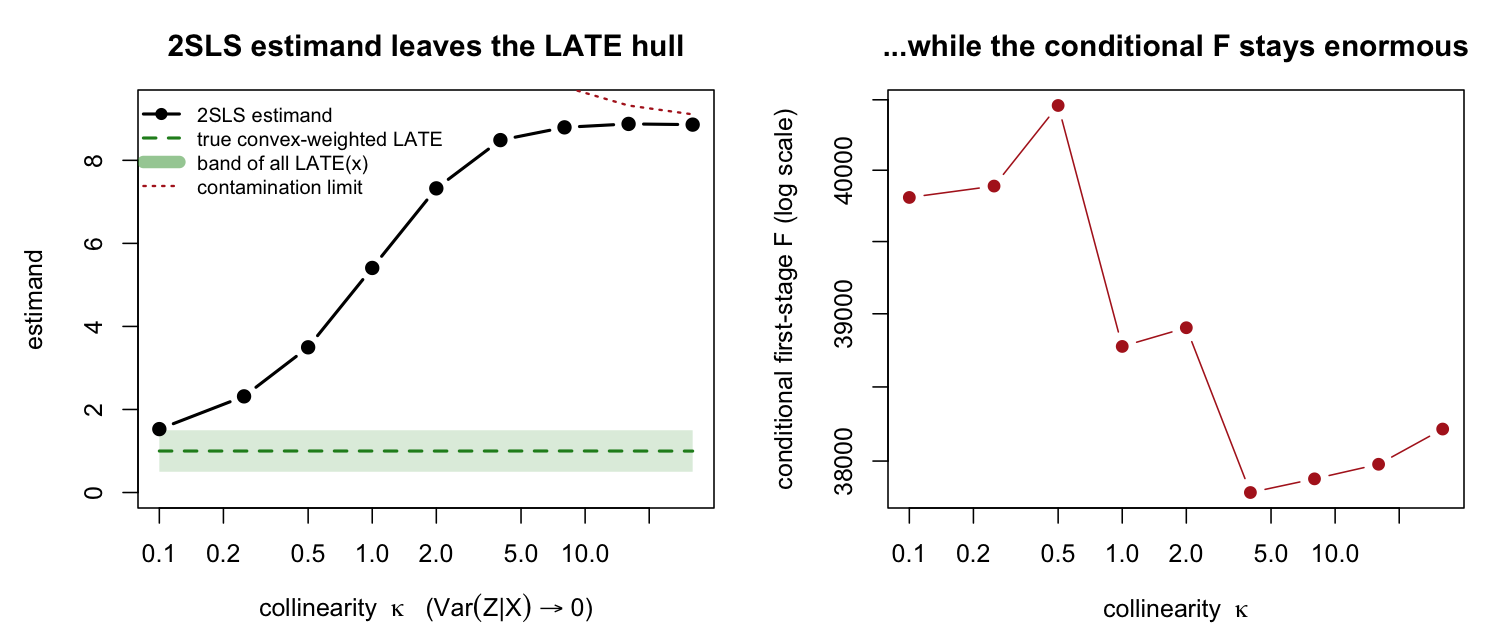
\includegraphics[width=\textwidth]{../figures/iv_collinearity_fig.png}
\caption{Left panel. As collinearity $\kappa$ rises, the 2SLS estimand (solid)
leaves the band of all conditional LATEs (shaded) and departs from the true
convex-weighted LATE (dashed), converging to the contamination limit (dotted).
Right panel. The conditional first-stage $F$ (log scale) stays near $\num{40000}$
throughout, far above the weak-IV threshold of $10$.}
\label{fig:collin}
\end{figure}

\subsection{Size and power}
Two exercises confirm the test's basic behaviour. Both are collected in
\ref{app:mc}. On a single large contaminated dataset ($n=\num{100000}$,
$\kappa=4$) the directed test rejects at $p<10^{-4}$ while the conditional $F$ is
$\num{20723}$, and the bias-corrected estimator recovers the true convex-weighted
LATE (Table~\ref{tab:sizepower}). Over $300$ replications at $n=3000$ it has a
conservative size of $1.3\%$ against the $5\%$ level under a linear propensity, and
power essentially one under a curved one, at
a mean conditional $F$ near $575$ in \emph{both} cases. The $F$ cannot discriminate
the two designs the test separates almost perfectly. A power sweep
(Table~\ref{tab:power}, Figure~\ref{fig:power}) raises the induced bias from $0$ to
$2.68$ while the mean conditional $F$ stays pinned near $\num{1740}$.

\subsection{Head-to-head comparison across three designs}\label{sec:head}
Table~\ref{tab:head} and Figure~\ref{fig:head} compare three procedures across
three designs at $n=3000$. The first procedure is a Ramsey RESET testing
curvature of the propensity $Z\sim X$, a functional of $(Z,X)$ alone. The second
is the strongly identified screening test of Section~\ref{sec:test}
($H_0:\theta_D=\theta_Y=0$), which we label ``Directed-S''. The third is the
bias-targeting test \eqref{eq:exactnull} of Section~\ref{sec:exact}, labelled
``Directed-X''. The \emph{contaminated} design has a nonlinear propensity and a
nonlinear outcome, so it carries real bias. The \emph{harmless} design has a
nonlinear propensity but a linear outcome and a homogeneous effect, so the bias
is zero despite strong curvature. The \emph{clean} design has a linear propensity
and zero bias. All three designs carry a mean conditional $F$ near $600$.

The pattern illustrates Proposition~\ref{prop:impossible}. In the
harmless design the RESET rejects $100\%$ of the time. It detects the propensity
curvature but, being blind to the outcome, cannot tell that the curvature is
inconsequential, and the same $F\approx600$ that accompanies a large bias in the
contaminated design accompanies zero bias here. Directed-S also false-alarms
($100\%$), because it tests the sufficient, not the necessary, condition. Only
Directed-X separates the three designs as the theory requires. It has full power
against genuine contamination, yet holds size ($4.7\%$) in the harmless design that
the other two procedures, and the conditional $F$, cannot certify. In the clean
design its rejection rate is $8.3\%$, about $2.6$ null standard errors above the
$5\%$ level at $300$ replications, a mild finite-sample over-rejection that the
larger-$n$ power curve (Table~\ref{tab:power}, where the $b=0$ size falls to
$0.5$--$1.0\%$ by $n\ge3000$) does not carry. We therefore read Directed-X as
correctly sized against harmless curvature and mildly liberal on a small-sample
clean design, not as exactly calibrated in finite samples.

\begin{table}[t]\centering
\caption{Head-to-head rejection rates ($5\%$ level, $300$ replications,
$n=3000$, cubic basis, $B=99$). ``mean cond.\ $F$'' is the average
Sanderson--Windmeijer conditional first-stage $F$.}
\label{tab:head}
\begin{tabular}{lcccc}
\toprule
design & RESET & Directed-S & Directed-X & mean cond.\ $F$\\
\midrule
CONTAMINATED (bias $\neq0$) & 1.00 & 1.00 & 1.00 & 602\\
HARMLESS \ \ \ (bias $=0$)  & 1.00 & 1.00 & \textbf{0.047} & 602\\
CLEAN \ \ \ \ \ \ \ (bias $=0$) & 0.06 & 0.013 & 0.083 & 572\\
\bottomrule
\end{tabular}
\end{table}

\begin{figure}[t]\centering
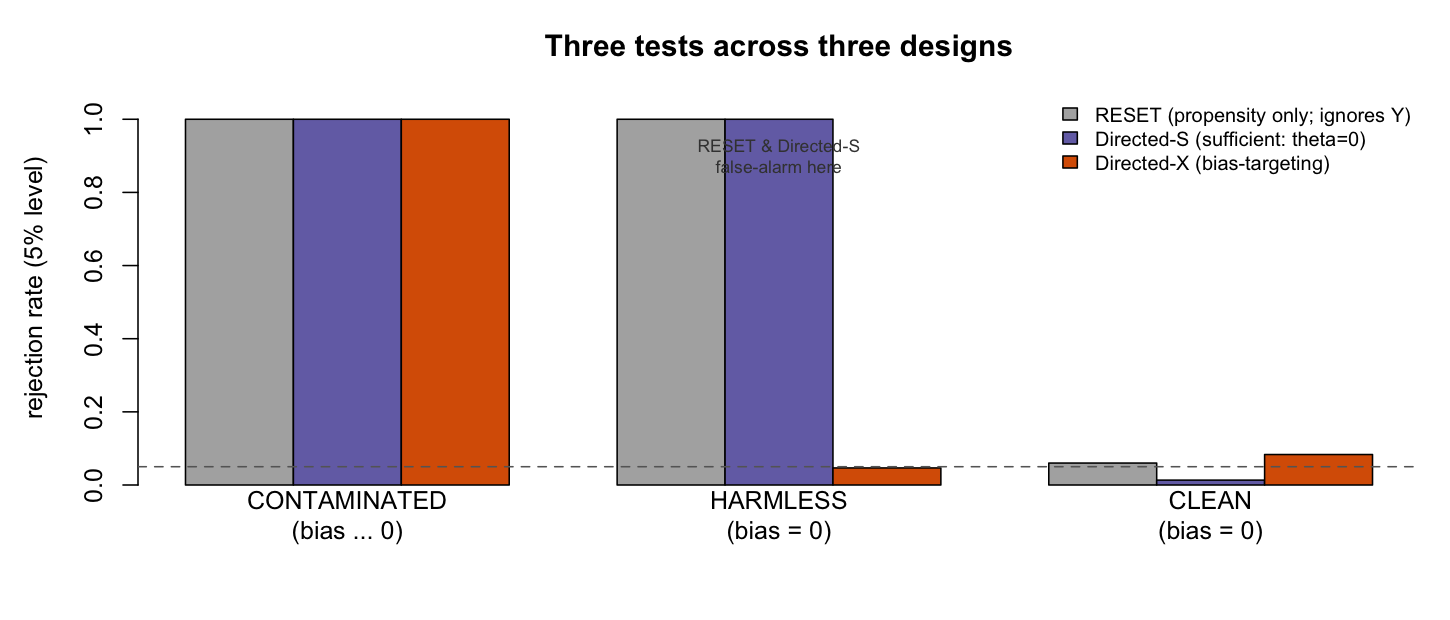
\includegraphics[width=\textwidth]{../figures/iv_headtohead.png}
\caption{Rejection rates of the RESET, the sufficient (Directed-S) and the
bias-targeting (Directed-X) tests across the contaminated, harmless, and clean
designs. In the harmless design (middle group) the RESET and Directed-S
false-alarm while Directed-X holds size, and the conditional $F$ (near $600$ in
all groups) cannot discriminate.}
\label{fig:head}
\end{figure}

Table~\ref{tab:svx} in \ref{app:mc} pushes the same contrast along the
collinearity knob. Both directed tests keep full power against genuine bias as
$\Var(Z\mid X)$ falls by an order of magnitude, so neither loses power to
collinearity. They part company only in the harmless design. There Directed-S
false-alarms every time, because its \emph{sufficient} condition $\theta=0$ is
false whenever the propensity is nonlinear, while Directed-X controls size
throughout, if anything conservatively, the pairs bootstrap insulating it from the
loss of pivotality that Corollary~\ref{cor:frontier} anticipates. This is the content of the ``report
both'' recommendation. Directed-S is a cheap screen that, at the cubic basis used
here, misses no contamination in the probed directions but cannot vindicate harmless
curvature, and Directed-X is the adjudicator that, in those same directions,
separates harmful from harmless. Both guarantees are relative to the fixed basis, per
Remark~\ref{rem:power}. A growing or orthogonalized basis extends them to all
directions.

\subsection{Estimating the contamination share}\label{sec:shareMC}
Table~\ref{tab:share} and Figure~\ref{fig:share} in \ref{app:mc} validate
the share estimator \eqref{eq:share}. The plug-in $\hat\varrho$ at $n=3000$ tracks
the population share from $\varrho\approx0.02$ to $\varrho\approx0.75$ with
$92$--$96\%$ bootstrap coverage. Because the bias also loads on the outcome-side
term, a modest share can coincide with substantial bias. At $\varrho=0.02$ the
estimand is already displaced by $1.3$ here. Thus $\hat\varrho$ flags manufactured
strength, while the test of Section~\ref{sec:exact} adjudicates its consequences.

%=============================================================================
\section{Empirical application}\label{sec:empirics}
%=============================================================================

We apply the diagnostic to a panel of canonical just-identified IV designs and
report all of them. The panel spans the three behaviours the theory predicts. The
first is a strong-instrument design whose linear-covariate estimate is materially
biased and which the correction repairs (Section~\ref{sec:401k}). The second is a
set of designs with genuine but harmless propensity curvature that the screening
test detects and the bias-targeting test correctly clears
(Section~\ref{sec:harmless}). The third is a set of designs the diagnostic clears
outright (Section~\ref{sec:clears}). Throughout, the flexible propensity uses a
low-order polynomial (or spline) basis and inference uses the pairs bootstrap of
Section~\ref{sec:test}.

A scope caveat governs how these results should be read. The binary-instrument,
binary-treatment model of Section~\ref{sec:framework} holds exactly for the headline
401(k) design (eligibility and participation are both binary) and for the Catholic
and Card designs, which have binary instruments. The remaining designs use the
instrument and treatment in their native multivalued or continuous form. Maimonides
predicted and actual class size, the Cornwell--Trumbull offense mix and arrest
probability, and the schooling designs' years of education are not dichotomized. The
reduced-form objects the diagnostic actually computes, namely the curvature
$h=e-L(e\mid1,X)$, the contamination moments $\theta_D=\E[h D]$ and
$\theta_Y=\E[h Y]$, the share $\varrho$, and the two directed tests, are functionals
of $\E[Z\mid X]$ and the level functions alone. They are therefore well defined and,
by the arguments of Sections~\ref{sec:test}--\ref{sec:correction}, retain their size
and consistency for a general $Z$ and $D$, since none of those arguments uses the
binary structure. What the binary model buys is the \emph{interpretation} of the
signal ratio $\bar L=S_Y/S_D$ as a convex average of conditional LATEs, through the
Wald--LATE identity of Lemma~\ref{lem:decomp}. For a multivalued instrument or
treatment $\bar L$ is instead the saturated-propensity linear-IV estimand, a
Blandhol-type weighted average of causal responses whose convexity requires the
multivalued monotonicity conditions we do not impose here. For those designs the
tests should accordingly be read as detecting, or certifying the absence of,
functional-form contamination of the linear-covariate 2SLS estimand relative to its
saturated-propensity counterpart, not as a statement about a convex-LATE object. The
multivalued convex-LATE decomposition is the open frontier of
Section~\ref{sec:conclusion}.

\subsection{A misleading strong first stage in the 401(k) design}\label{sec:401k}

Our headline application is the effect of 401(k) participation on household net
financial assets, using 401(k) \emph{eligibility} as an instrument for
participation \citep{poterba1995,abadie2003}. We use the cross-section of
$n=9{,}275$ households of \citet{wooldridge2010}. Eligibility is an extremely
strong instrument, with a conditional first-stage $F$ exceeding $7{,}000$. But
firms offer eligibility in a manner strongly nonlinear in income, and income is a
first-order, nonlinear determinant of wealth. This is precisely the configuration
of Lemma~\ref{lem:decomp} in which linear covariate adjustment contaminates the
estimand.

Table~\ref{tab:401k} reports the just-identified 2SLS estimate (participation on
net financial assets, in thousands of dollars) under three income
specifications, with the diagnostic.\footnote{Full specification, from the released
\texttt{iv\_401k.R}. Treatment $D$ is 401(k) participation, instrument $Z$ is 401(k)
eligibility, outcome $Y$ is net financial assets. The linear control vector is
(income, age, married, male, family size). The curvature basis $b(X)$ for the linear
specification is $(\mathrm{inc}^2,\mathrm{inc}^3,\mathrm{age}^2,\mathrm{inc}\times
\mathrm{age})$ residualized against the linear controls. The quadratic specification
adds $\mathrm{inc}^2,\mathrm{age}^2$ to the controls with basis
$(\mathrm{inc}^3,\mathrm{inc}^4,\mathrm{age}^3,\mathrm{inc}\times\mathrm{age})$. The
spline robustness check uses a natural-spline income basis with six degrees of
freedom, and the flexible benchmark controls income and age by natural splines with
five and four degrees of freedom. Inference is a pairs bootstrap with $B=1499$
resamples that refits the propensity, the curvature basis, and the level functions on
each resample.} Under a \emph{linear} income control, a
common and parsimonious default, the estimate is $8.40$. Both the screening and
the bias-targeting tests reject decisively ($p<10^{-3}$) \emph{despite}
$F>7{,}000$, and the bias-corrected estimand is $12.6$ ($[9.0,16.0]$). The
correction is validated in three ways. Controlling income \emph{quadratically}
removes the flag ($p_X=0.11$) and gives $13.7$. A flexible natural-spline income
control gives $13.1$. Our correction from the linear specification, $12.6$,
coincides with both. The naive linear-income estimate is the outlier,
understating the effect by roughly a third. The rejection is robust to the
curvature basis, since polynomial and natural-spline bases both give
$p_X<10^{-3}$, and it is self-validating, since it disappears exactly when income
is controlled flexibly.

\begin{table}[t]\centering
\caption{The 401(k) design ($n=9{,}275$). Effect of participation on net financial
assets (\$000s), instrumented by eligibility. A first-stage $F>7{,}000$ does not
prevent contamination under linear income control, and the correction recovers the
flexible-income answer. Test $p$-values from the pairs bootstrap. For the corrected
row, cond.\ $F$ is the corrected estimator's own first stage (regressing $D$ on the
residualized instrument $Z-\hat e(X)$), the bracketed interval is the pairs
bootstrap, and its identification-robust Anderson--Rubin $95\%$ interval is
$[8.2,17.0]$.}
\label{tab:401k}
\resizebox{\textwidth}{!}{%
\begin{tabular}{lccccc}
\toprule
income control & 2SLS effect & cond.\ $F$ & $\hat\varrho$ & Directed-S $p$ & Directed-X $p$\\
\midrule
linear (naive) & 8.40 & 7401 & 0.03 & $<0.0001$ & $0.0001$\\
quadratic & 13.66 & 7423 & 0.00 & 0.121 & 0.113\\
natural splines (benchmark) & 13.05 & n/a & n/a & n/a & n/a\\
\emph{contamination-corrected} & \emph{12.6 [9.0, 16.0]} & \emph{7295} & & & \\
\bottomrule
\end{tabular}}
\end{table}

This is the paper's thesis on real data. A first-stage $F$ above seven thousand
offers no protection. Under linear income control the estimand is contaminated by
the covariance between the eligibility propensity's income curvature and the steep
income profile of wealth. By Proposition~\ref{prop:impossible} no first-stage
diagnostic could reveal this, and none does. Both numbers computed from the first
stage, the conditional $F>7{,}000$ and the contamination share $\hat\varrho=0.03$,
report a clean, strongly identified design. They miss the bias because here it
loads on the outcome side, through $\theta_Y$ rather than the first-stage term
$\theta_D$, the channel no relevance diagnostic can reach. Only the outcome-based
directed test detects it, and the correction returns the specification-robust
answer. The 401(k) design is thus failure mode~(b) in near-pure form. The strength
is honest and overwhelming, and with $\hat\varrho=0.03$ the bias is
\emph{predominantly} on the outcome side. Decomposing the displacement of $8.4$ from
the corrected $12.6$, the first-stage channel $-\bar L\,\hat\varrho$ accounts for
only about a tenth of it and the outcome term $\theta_Y$ for the rest, so the
first-stage numbers see essentially none of the bias. It is the empirical face of
Proposition~\ref{prop:impossible}.
The very design in which every first-stage number is reassuring is the one that is
biased.

The corrected estimand still needs an interval. Proposition~\ref{prop:tradeoff}
warns that de-contamination can destroy identification, so a corrected point
estimate must be read with an interval that is robust to weak identification. Here
that caveat does not bind. Because the contamination share is only
$\hat\varrho=0.03$, the corrected estimator retains almost all of the first-stage
covariance, and its \emph{own} first-stage $F$ (regressing $D$ on the residualized
instrument $Z-\hat e(X)$) is $\num{7295}$. The corrected estimator is therefore
strongly identified, and the identification-robust Anderson--Rubin $95\%$ interval,
$[8.2,17.0]$, is bounded and coincides with the normal-theory interval, confirming
that the pairs-bootstrap interval $[9.0,16.0]$ is valid in this design. The general
rule follows recommendation~(3). When $\hat\varrho$ is small the corrected first
stage survives and standard or bootstrap intervals apply, whereas when $\hat\varrho$
approaches one the corrected first stage collapses and the interval must be read off
the Anderson--Rubin set rather than the bootstrap. The careful applied literature avoids the
problem by controlling income flexibly, which is exactly what the correction
reproduces. The contribution is a diagnostic that flags the common parsimonious
specification that does not do so, and that a large $F$ would otherwise excuse.

\subsection{Genuine but harmless curvature}\label{sec:harmless}

Two further strong-instrument designs show the value of separating the screening
test from the bias-targeting test (Table~\ref{tab:harmless}). In the class-size
design of \citet{angrist1999}, the instrument is Maimonides' rule predicted class
size, a deterministic sawtooth in enrollment. The conditional $F$ is $458$ and the
screening test rejects decisively ($\hat\varrho=0.23$, $p<10^{-4}$), so a large
part of the apparent strength is propensity curvature, invisible to the $F$. Yet
the bias-targeting test does \emph{not} reject ($p_X=0.19$). The correction moves the
math estimate from $-0.171$ to $-0.217$. That shift is sizeable in proportional
terms, but the bias-targeting $p$-value shows it is not statistically distinguishable
from zero at the cubic basis, so the design is certified as harmless-curvature rather
than as numerically unchanged. A schooling IV using father's education
\citep{wooldridge2010} behaves the same way, with a much smaller point shift. These
are real-data instances of the harmless-curvature case of Section~\ref{sec:head},
read at cubic order per Remark~\ref{rem:power}.

\begin{table}[t]\centering
\caption{Strong-instrument designs with genuine but harmless curvature. The
screening test rejects (curvature present) but the bias-targeting test clears and
the correction $\approx$ the naive estimate.}
\label{tab:harmless}
\resizebox{\textwidth}{!}{%
\begin{tabular}{lcccccc}
\toprule
design & $n$ & cond.\ $F$ & $\hat\varrho$ & Directed-S $p$ & Directed-X $p$ & naive\,$\to$\,corr.\\
\midrule
Maimonides, math       & 2013 & 458 & 0.23 & $<0.0001$ & 0.19 & $-0.171\to-0.217$\\
Maimonides, verbal     & 2013 & 458 & 0.23 & $<0.0001$ & 0.75 & $-0.221\to-0.230$\\
Schooling, father's educ. & 741 & 95 & 0.15 & 0.001 & 0.18 & $\phantom{-}0.110\to0.119$\\
\bottomrule
\end{tabular}}
\end{table}

\subsection{Designs the diagnostic clears}\label{sec:clears}

Table~\ref{tab:clears} reports the remaining eight designs. Among them are schooling
instrumented by college proximity \citep{card1995} and by mother's education
\citep{mroz1987}, the institutions--income IV \citep{acemoglu2001} (inconclusive at
$n=64$), openness--inflation \citep{romer1993}, and the Cornwell--Trumbull crime IV
\citep{cornwell1994}. All clear both tests, with a corrected estimand
indistinguishable from the linear-covariate 2SLS estimate. The diagnostic does not
manufacture false alarms. These non-rejections are at cubic order, and by
Remark~\ref{rem:power} certify only that no contamination is detectable in the
probed directions, not its absence in every direction.

\begin{table}[t]\centering
\caption{Designs the diagnostic clears (both tests $p>0.10$, corrected $\approx$
naive). The contamination share $\hat\varrho$ is small except at AJR, which is reported
as inconclusive given $n=64$.}
\label{tab:clears}
\resizebox{\textwidth}{!}{%
\begin{tabular}{lccccc}
\toprule
design & $n$ & cond.\ $F$ & $\hat\varrho$ & Directed-S $p$ & Directed-X $p$\\
\midrule
Schooling, college proximity (Card)      & 3010 & 14  & 0.03 & 0.74 & 0.81\\
Schooling, mother's educ.\ (Mroz)        & 428  & 73  & 0.02 & 0.83 & 0.74\\
Cigarette demand, taxes                   & 48   & 326 & 0.02 & 0.85 & 0.79\\
Institutions, settler mortality (AJR)     & 64   & 12  & 0.21 & 0.19 & 0.98\\
Openness--inflation, log land (Romer)     & 114  & 44  & 0.00 & 0.97 & 0.79\\
Botswana fertility, birth timing          & 4358 & 43  & 0.00 & 0.91 & 0.97\\
Catholic schooling, parent Catholic       & 7430 & 389 & 0.01 & 0.12 & 0.25\\
Crime, offense mix (Cornwell--Trumbull)   & 630  & 105 & 0.00 & 0.56 & 0.31\\
\bottomrule
\end{tabular}%
}
\end{table}

Across the panel the diagnostic behaves as designed. It flags and repairs a
consequential contamination in a design with an overwhelming first stage (401(k),
mode~b), detects genuine curvature that it then correctly certifies harmless
(Maimonides, schooling by father's education), and clears the remaining designs.
That well-identified published designs largely clear the bias-targeting test is not
evidence that the problem is rare. It is evidence that the diagnostic is
\emph{specific}, in that it does not manufacture alarms on clean designs, the
property a RESET lacks (Section~\ref{sec:head}). The 401(k) case shows the converse,
that a large first-stage $F$ is no guarantee, and that the contamination it conceals
is both detectable and correctable.

%=============================================================================
\section{Recommendations for practice}\label{sec:practice}
%=============================================================================

Our results imply a short protocol that adds little cost to a standard IV
analysis. (1) Report the \emph{conditional} first-stage $F$ of
\citet{sanderson2016}, but do not treat it as evidence for a causal reading of
the second stage, and report the estimated contamination share
$\hat\varrho$~\eqref{eq:share} beside it. (2) Estimate the instrument propensity
$\E[Z\mid X]$ flexibly and test its curvature against $D$ and $Y$ using the
screening statistic of Section~\ref{sec:test} and, to distinguish harmful from
harmless curvature, the bias-targeting test of Section~\ref{sec:exact}. A screening
rejection signals curvature that loads on $D$ and $Y$ even when the conditional $F$
is large, but it does not by itself establish bias. Use the bias-targeting test to
decide. (3) If the \emph{bias-targeting} test rejects, report the bias-corrected
estimand~\eqref{eq:correction} together with weak-IV-robust inference, and
recognize (Proposition~\ref{prop:tradeoff}) that a collapse in the corrected
first stage means the apparent strength was contamination rather than
identification. A screening rejection that the bias-targeting test does not confirm
is the harmless-curvature case and calls for no correction. (4) Where feasible, prefer an instrument whose propensity is
approximately linear in the controls, or saturate the controls at the design
stage while monitoring the resulting conditional strength.

%=============================================================================
\section{Conclusion}\label{sec:conclusion}
%=============================================================================

The applied ritual of reporting a first-stage $F$ answers whether an instrument
moves the treatment, not whether the second-stage estimate is a meaningful causal
average. Under instrument--covariate collinearity these questions come apart in a
specific, detectable way. The same propensity curvature that contaminates the
linear-covariate 2SLS estimand also inflates the conditional $F$, so the strength
diagnostic cannot see the problem and the natural saturation fix trades the bias
for weak identification. A directed conditional-moment test, built entirely from
reduced-form regressions, has power exactly where the conditional $F$ is silent.

The analysis is deliberately confined to a binary instrument, a binary treatment,
and just identification. We now say what survives beyond that boundary and what does
not. Overidentification is the benign direction, though it is less mechanical than a
single reduced form. With a vector of instruments the FWL numerator and denominator
of Lemma~\ref{lem:decomp} each become a curvature--level covariance vector, one entry
per instrument, but the 2SLS estimand combines them through the
residualized-instrument second-moment matrix, so the population coefficient is a
weighted combination of the per-instrument signal and contamination vectors rather
than a clean term-by-term ratio. What does carry over exactly is the diagnostic
content. The impossibility result (Proposition~\ref{prop:impossible}) holds
verbatim, since the bias still loads on the outcome, and the directed test extends by
stacking the moments $\E[h_j(X)D]$ and $\E[h_j(X)Y]$ across instruments $j$ and
testing them jointly. The stacked moment restriction is a sufficient screen for no
contamination. An exact overidentified analogue of the bias-targeting restriction,
which must invert the second-moment matrix, we leave to future work.
Multiple or multivalued treatments are the substantive frontier. There our
single-treatment, functional-form contamination compounds with the
\emph{cross-treatment} contamination of \citet{goldsmith2024}, a conceptually
distinct channel that persists even under a saturated propensity, and disentangling
the two is genuinely open. What extends cleanly in every case is the reason the
first stage cannot help. The bias always loads on the conditional law of the
outcome, so Proposition~\ref{prop:impossible} is not special to the binary model.
The remaining loose end, a data-driven curvature basis, is closed by
Proposition~\ref{prop:orthogonal}. We leave the multivalued extension to future
work, where the object to be tested is a matrix rather than a scalar contamination.

%=============================================================================
\appendix
\section{Proofs}\label{app:proofs}
%=============================================================================

\subsection*{Proof of Lemma~\ref{lem:decomp}}
By \eqref{eq:fwl}, $\beta_{2SLS}=\E[\Ztil Y]/\E[\Ztil D]$ with
$\Ztil=Z-\ell(X)$. Write $\Ztil=(Z-e(X))+h(X)$ using $h=e-\ell$. For any
integrable $W\in\{D,Y\}$,
\[
\E[\Ztil W]=\E[(Z-e(X))W]+\E[h(X)W].
\]
For the first term, condition on $X$. Since $\E[Z-e(X)\mid X]=0$, we have
$\E[(Z-e(X))W\mid X]=\Cov(Z,W\mid X)$. For binary $Z$,
$\Cov(Z,W\mid X)=e(X)\{1-e(X)\}\{\E[W\mid Z=1,X]-\E[W\mid Z=0,X]\}$. For $W=D$
this contrast is $p(X)$. For $W=Y$, Assumptions~\ref{as:valid}--\ref{as:rel} give
the conditional Wald identity
$\E[Y\mid Z=1,X]-\E[Y\mid Z=0,X]=p(X)\late(X)$. Taking expectations over $X$
yields $S_D$ and $S_Y$. For the second term,
$\E[h(X)W]=\E[h(X)\E[W\mid X]]=\E[h(X)m_W(X)]=\Cov(h(X),m_W(X))$, the last
equality because $\E[h(X)]=0$. This gives $\theta_D,\theta_Y$ and
\eqref{eq:decomp}. Equation~\eqref{eq:bias} follows by subtracting
$\bar L=S_Y/S_D$ from \eqref{eq:decomp} and simplifying, and
$S_D+\theta_D=\E[\Ztil D]$ by construction. \hfill$\qed$

\subsection*{Proof of Proposition~\ref{prop:collin}}
By Assumption~\ref{as:seq}(i), $e_t(1-e_t)\to0$ a.e.\ and in $L^1$. For $S_{D,t}$,
$0\le e_t(1-e_t)p_t\le\frac14$ since $p_t\in[0,1]$, so bounded convergence gives
$S_{D,t}=\E[e_t(1-e_t)p_t]\to0$. For $S_{Y,t}$ the integrand
$e_t(1-e_t)p_t\late_t\to0$ a.e., and no fixed envelope dominates it because $\late_t$
varies with $t$. We instead invoke Vitali's theorem. The family is uniformly
integrable because $|e_t(1-e_t)p_t\late_t|\le\frac14|\late_t|$ and $\late_t\to
\late^\ast$ in $L^2$, so $\{\late_t\}$ is $L^1$-uniformly integrable, giving
$S_{Y,t}=\E[e_t(1-e_t)p_t\late_t]\to0$. By
Assumption~\ref{as:seq}(ii)--(iii), $h_t\to h^\ast$ and $m_{D,t},m_{Y,t}$
converge in $L^2$, so by Cauchy--Schwarz
$\theta_{D,t}=\Cov(h_t,m_{D,t})\to\Cov(h^\ast,m_D^\ast)$ and likewise
$\theta_{Y,t}\to\Cov(h^\ast,m_Y^\ast)$. The denominator of
\eqref{eq:decomp} converges to $\Cov(h^\ast,m_D^\ast)$, nonzero by
Assumption~\ref{as:seq}(iv), so \eqref{eq:limit} follows from the continuous
mapping theorem. That the limit can fall outside the LATE hull or flip sign is
shown by the construction in Section~\ref{sec:mc}, where all $\late(x)>0$ yet the
limit exceeds $\sup_x\late(x)$. \hfill$\qed$

\subsection*{Proof of Corollary~\ref{cor:Ffails}}
The population conditional first-stage slope from regressing $D$ on $\Ztil$ is
$\pi_t=\E[\Ztil_t D]/\Var(\Ztil_t)$. By Lemma~\ref{lem:decomp},
$\E[\Ztil_t D]=S_{D,t}+\theta_{D,t}\to\Cov(h^\ast,m_D^\ast)$, and
$\Var(\Ztil_t)=\E[e_t(1-e_t)]+\E[h_t^2]\to\E[(h^\ast)^2]$ by
Assumption~\ref{as:seq}(i)--(ii). Hence
$\pi_t\to\Cov(h^\ast,m_D^\ast)/\E[(h^\ast)^2]\neq0$. The conditional $F$ has
population analogue $n\,\pi_t^2\,\Var(\Ztil_t)/\sigma^2_v$ with
$\sigma^2_v=\Var(D-\pi_t\Ztil-X'c)$ bounded, so it is bounded away from zero and
diverges in $n$. \hfill$\qed$

\subsection*{Proof of Proposition~\ref{prop:impossible}}
Fix the joint law of $(Z,D,X)$ with $h\neq0$. Then $e(\cdot)$, $\ell(\cdot)$,
$h(\cdot)$, $m_D(\cdot)$, $p(\cdot)$, $S_D=\E[e(1-e)p]$, $\theta_D=\E[h(X)D]$ and
$\Var(\Ztil)$ are all determined, so any functional $T$ of this law takes a fixed
value. By \eqref{eq:bias}, $\beta_{2SLS}-\bar L=(\theta_Y-\bar L\theta_D)/
(S_D+\theta_D)$ with $\theta_Y=\E[h(X)Y]$ and
$\bar L=S_Y/S_D$, $S_Y=\E[(Z-e(X))Y]$. Both $\theta_Y$ and $S_Y$ are determined
by the conditional law of $Y$ given $(Z,X)$, which is not restricted by the
marginal law of $(Z,D,X)$. Construct two outcome laws sharing that marginal but
with conditional means $m_Y$ and $m_Y'$ that differ on the span orthogonal to
$(1,X')$, i.e.\ $\Cov(h,m_Y)\neq\Cov(h,m_Y')$. Because $h\neq0$ such a perturbation
exists. The perturbation changes only the level $\E[Y(d)\mid X]$ of the potential
outcomes and leaves $D=D(Z)$, the treatment law, and the conditional LATEs
untouched, so Assumptions~\ref{as:valid}--\ref{as:rel} are preserved and both DGPs
are admissible IV models. Then the two biases differ while $T$ is identical across
them. Since the gap $\Cov(h,m_Y)-\Cov(h,m_Y')$ can be made arbitrarily large (scale
the orthogonal component of $m_Y'$), the bias is unbounded as a function of the
outcome law at fixed $T$. Hence $T$ carries no information about the bias. When
$h\equiv0$ the construction is empty because $\Cov(h,\cdot)\equiv0$, consistent with
the first stage then certifying no contamination. \hfill$\qed$

\subsection*{Proof of Proposition~\ref{prop:test}}
$\hat\theta$ is a two-step estimator, a first-step OLS $\hat\delta$ from
regressing $Z$ on $(1,X',b(X)')$, and second-step sample means of $\hat h_i W_i$,
$W\in\{D,Y\}$. Under the stated moment conditions and fixed $K$,
$\hat\delta\convp\delta$ and is asymptotically linear with influence
$G^{-1}b(X_i)u_i$, $G=\E[bb']$. A mean-value expansion of
$\hat\theta_W=n^{-1}\sum_i b(X_i)'\hat\delta\,W_i$ around $\delta$ gives
$\sqrt n(\hat\theta_W-\theta_W)=n^{-1/2}\sum_i\{b(X_i)'\delta\,W_i-\theta_W\}
+\E[W b(X)']\sqrt n(\hat\delta-\delta)+o_p(1)$, which is the influence function
stated. The central limit theorem yields
$\sqrt n(\hat\theta-\theta)\convd N(0,\Sigma)$ with
$\Sigma=\Var(\psi_i)$. Under $H_0$, $\theta=0$ and $W_n=n\hat\theta'\hat\Sigma^{-1}
\hat\theta\convd\chi^2_2$ provided $\hat\Sigma\convp\Sigma\succ0$. Consistency
against fixed alternatives and the local power statement are immediate from
$\hat\theta\convp\theta\neq0$ and $\theta=\eta/\sqrt n$, respectively.
Consistency of the pairs bootstrap for $\Sigma$ follows from Hadamard
differentiability of $\hat\theta$ in the empirical measure. \hfill$\qed$

\subsection*{Proof of Proposition~\ref{prop:weakrobust}}
Fix a sequence $\{P_n\}$ as stated. The estimator $\hat\theta$ and its influence
function
$\psi_{i}=(b(X_i)'\delta\,W_i-\theta_W)_{W\in\{D,Y\}}+\big(\E[Wb(X)']\big)_W G^{-1}b(X_i)u_i$
from the proof of Proposition~\ref{prop:test} involve the first-stage strength
nowhere. They are determined by the reduced-form regression of $Z$ on
$(1,X',b(X)')$ and by the cross-moments $\E[Wb(X)']$, none of which is the
first-stage covariance $\E[\Ztil D]$. The weak-instrument problem is a
small-denominator problem for $\beta_{2SLS}=\E[\Ztil Y]/\E[\Ztil D]$, and that
denominator does not appear. The uniform fourth-moment bound and
$\Sigma_n\to\Sigma_\ast\succ0$ posited for the null sequence supply a Lyapunov
condition, so the Lindeberg--Feller central limit theorem for triangular arrays
applies to $n^{-1/2}\sum_i\psi_{i,n}$, giving
$\sqrt n(\hat\theta-\theta)\convd N(0,\Sigma_\ast)$ along the sequence. Under $H_0$,
$\theta=0$ and $\hat\Sigma\convp\Sigma_\ast$, so $W_n\convd\chi^2_2$. The
generated-regressor term $\E[Wb(X)']G^{-1}b(X_i)u_i$ has variance of order
$\Var(u_i)\to0$ as $Z$ becomes collinear, but the leading term
$b(X_i)'\delta\,W_i-\theta_W$ has variance bounded below because the curvature stays
nondegenerate, $h_n\to h^\ast\neq0$ and hence $\delta\to\delta^\ast\neq0$. This
delivers $\Sigma_\ast\succ0$. The identical argument applied to the orthogonalized
influence $\psi^o_i$, which is likewise free of the first-stage covariance, gives
$W^o_n\convd\chi^2_2$. Finally, along the contaminated sequence of
Assumption~\ref{as:seq} the same central limit theorem gives
$\sqrt n(\hat\theta-\theta_n)\convd N(0,\Sigma_\ast)$ while $\theta_n\to\theta^\ast$
with $\theta_D^\ast=\Cov(h^\ast,m_D^\ast)\neq0$; the noncentrality
$n\,\theta_n'\Sigma_n^{-1}\theta_n\to\infty$, so $W_n\to\infty$ in probability and
the power tends to one. \hfill$\qed$

\subsection*{Proof of Proposition~\ref{prop:orthogonal}}
Mean zero at the truth is immediate, because
$\E[\psi^o_W]=\E[h(X)W]+\E[\tilde m_W(X)(Z-e(X))]-\theta_W=\theta_W+0-\theta_W=0$,
using $\E[Z-e(X)\mid X]=0$. For orthogonality with respect to $e$, perturb
$e\to e+t\Delta$. Because $h=e-L(e\mid1,X)$ is linear in $e$ and the linear
projection is self-adjoint,
$\partial_t\E[h(X)W]\big|_{t=0}=\E[(\Delta-L(\Delta\mid1,X))\,m_W(X)]
=\E[\Delta\,\tilde m_W(X)]$, while
$\partial_t\E[\tilde m_W(X)(Z-e(X))]\big|_{t=0}=-\E[\tilde m_W(X)\,\Delta(X)]$. The
two terms cancel. Perturbing $m_W\to m_W+t\,\Xi$ moves only the correction term,
with derivative $\E[\tilde\Xi(X)(Z-e(X))]=\E[\tilde\Xi(X)\,\E(Z-e(X)\mid X)]=0$.
Hence $\psi^o_W$ is Neyman-orthogonal in both nuisances. The affine projection
$L(\cdot\mid1,X)$ is not a third nuisance but a linear functional of $e$: the
$e$-perturbation above moves $h=e-L(e\mid1,X)$ through the projection, and the same
self-adjointness that makes the two derivatives cancel annihilates its first-order
contribution \emph{to the pathwise derivative}. In the estimator the projection is a
parametric $\sqrt n$ step, an OLS of $Z$ on $(1,X)$; its estimation error contributes
a regular $O_p(n^{-1/2})$ term to the influence function, not orthogonalized away but
asymptotically linear, which the pairs bootstrap captures by recomputing the
projection, the curvature basis, and the level functions on each resample. With $K$-fold cross-fitting the
plug-in decomposes as
$\hat\theta^o_W-\theta_W=n^{-1}\sum_i\psi^o_W(O_i;e,m_W)
+\text{(bias)}+\text{(remainder)}$. Orthogonality bounds the bias by the product
$\|\hat e-e\|_{L^2}\|\hat m_W-m_W\|_{L^2}=o_p(n^{-1/2})$, and cross-fitting makes
the remainder $o_p(n^{-1/2})$ under the stated $L^2$ rates and fourth moments
\citep{chernozhukov2018}. The leading term is a sample average of the fixed
influence $\psi^o_i$, so $\sqrt n(\hat\theta^o-\theta)\convd N(0,\Sigma_o)$ by the
central limit theorem, and $W^o_n\convd\chi^2_2$ under $H_0$ follows as in the
proof of Proposition~\ref{prop:test}. \hfill$\qed$

\subsection*{Proof of Propositions~\ref{prop:correction} and \ref{prop:tradeoff}}
Write the numerator of \eqref{eq:correction} as
$n^{-1}\sum_i(Z_i-\hat e(X_i))Y_i=n^{-1}\sum_i(Z_i-e(X_i))Y_i
-n^{-1}\sum_i(\hat e(X_i)-e(X_i))Y_i$. The first term converges in probability to
$\E[(Z-e(X))Y]=S_Y$ by the argument in the proof of Lemma~\ref{lem:decomp}. For
the second, by Cauchy--Schwarz its magnitude is at most
$(n^{-1}\sum_i(\hat e(X_i)-e(X_i))^2)^{1/2}(n^{-1}\sum_i Y_i^2)^{1/2}
=\|\hat e-e\|_{n}\cdot O_p(1)$, where $\|\hat e-e\|_{n}^2=n^{-1}\sum_i(\hat
e(X_i)-e(X_i))^2$ is the in-sample empirical norm. This is $o_p(1)$ whenever
$\|\hat e-e\|_{n}=o_p(1)$. For the fixed, low-dimensional basis used throughout,
the empirical norm converges to the population norm $\|\hat e-e\|_{L^2}$ by a
uniform law of large numbers, so mere $L^2$-consistency of the propensity estimator
suffices, with no orthogonality or rate requirement. For a flexible,
high-dimensional or machine-learning $\hat e$ trained in-sample, population
$L^2$-consistency need not control the empirical norm; one should then cross-fit
$\hat e$, evaluating it on observations not used to fit it, so that the displayed
average is genuinely out-of-sample and the argument goes through unchanged. The
denominator converges
to $\E[(Z-e(X))D]=S_D$ identically, and provided $S_D\neq0$ in the fixed
data-generating process the ratio converges to $S_Y/S_D=\bar L$, proving
Proposition~\ref{prop:correction}. (Asymptotic normality and inference for
$\hat{\bar L}$, as opposed to consistency, do require controlling the first-step
influence, for example a Neyman-orthogonalized moment with cross-fitting, and,
because $S_D$ may be small, weak-instrument-robust confidence sets. See
Remark~\ref{rem:np} and Section~\ref{sec:correction}.) For
Proposition~\ref{prop:tradeoff}, the corrected estimator's first-stage covariance
is exactly this denominator $\E[(Z-e(X))D]=S_D=\E[e(X)\{1-e(X)\}p(X)]$, which by
Proposition~\ref{prop:collin} tends to $0$ under Assumption~\ref{as:seq}. The
identity of Corollary~\ref{cor:frontier} is immediate: $\varrho=\theta_D/\E[\Ztil D]$
by \eqref{eq:share} and $S_D=\E[\Ztil D]-\theta_D$, so $S_D=(1-\varrho)\E[\Ztil D]$;
the concentration-parameter statement follows because the corrected instrument
$Z-e(X)$ has covariance $S_D$ with $D$ and variance $\E[e(1-e)]$. \hfill$\qed$

\subsection*{Asymptotics of the bias-targeting statistic $T_n^{\ast}$}
Let $\hat g=n^{-1}\sum_i\hat h_i(Y_i-\hat{\bar L}D_i)$ estimate
$g(\bar L)=\E[h(X)(Y-\bar L D)]$, which equals $\theta_Y-\bar L\theta_D$ and is
zero under $H_0^{\ast}$ by \eqref{eq:bias}. Expanding in $(\hat\delta,\hat{\bar L})$
about $(\delta,\bar L)$,
$\sqrt n\,\hat g=n^{-1/2}\sum_i\{h(X_i)(Y_i-\bar L D_i)-g(\bar L)\}
+\E[b(X)'(Y-\bar L D)]\,\sqrt n(\hat\delta-\delta)
-\theta_D\,\sqrt n(\hat{\bar L}-\bar L)+o_p(1)$.
We require, beyond Assumption~\ref{as:test} and $S_D$ bounded away from zero, that
$\hat{\bar L}$ be $\sqrt n$-asymptotically linear with an influence function
$\phi_i$, $\sqrt n(\hat{\bar L}-\bar L)=n^{-1/2}\sum_i\phi_i+o_p(1)$. This is a
genuine additional condition. Proposition~\ref{prop:correction} delivers only
consistency of $\hat{\bar L}$, so its asymptotic linearity must be supplied
separately, for instance by the Neyman-orthogonalized, cross-fitted estimator of
Proposition~\ref{prop:orthogonal} and Remark~\ref{rem:np} under those rate
conditions, which is why we invoke that construction rather than the plug-in when we
need an interval. Given it, $\sqrt n(\hat\delta-\delta)$ and
$\sqrt n(\hat{\bar L}-\bar L)$ are both asymptotically linear, so
$\sqrt n\,\hat g\convd N(0,v)$ for a finite $v>0$. In this fixed, strongly identified
data-generating process the pairs bootstrap is first-order valid for the smooth
functional $\hat g$ by the same Hadamard-differentiability argument as in
Proposition~\ref{prop:test}, so the bootstrap variance $\hat v$ satisfies
$n\hat v\convp v$. Then
$T_n^{\ast}=\hat g^2/\hat v=(\sqrt n\,\hat g)^2/(n\hat v)\convd\chi^2_1$
under $H_0^{\ast}$, and $\hat g\convp g(\bar L)\neq0$ gives consistency against any
fixed alternative with nonzero bias. (Equivalently, one may write the statistic as
$n\hat g^2/\hat v_1$ with $\hat v_1\convp v$ a consistent estimate of the asymptotic
variance of $\sqrt n\,\hat g$; the two forms coincide since $\hat v_1=n\hat v$.) As
$S_D\to0$ the term $-\theta_D\sqrt n(\hat{\bar L}-\bar L)$ ceases to be $O_p(1)$,
$\hat{\bar L}$ is no longer $\sqrt n$-consistent, and both the Gaussian limit and the
bootstrap approximation fail. We do not establish size control for $T_n^{\ast}$ at
that boundary. The favourable finite-sample behaviour over the collinearity range in
Table~\ref{tab:svx} is a simulation finding, not a proof of weak-signal validity, and
this is exactly why the protocol pairs $T_n^{\ast}$ with the screening test, whose
size is controlled along the collinearity sequence
(Proposition~\ref{prop:weakrobust}). \hfill$\qed$

%=============================================================================
\section{Additional Monte Carlo evidence}\label{app:mc}
%=============================================================================

This appendix collects the size-and-power, power-curve, collinearity-sweep, and
share-estimation exhibits summarized in Section~\ref{sec:mc}. The design is that of
Section~\ref{sec:mc}.

\begin{table}[h]\centering
\caption{Directed contamination test. Panel A, one dataset, $n=\num{100000}$.
Panel B, rejection rates, $5\%$ level, $300$ replications, $n=3000$, cubic basis.}
\label{tab:sizepower}
\begin{tabular}{lccccc}
\multicolumn{6}{l}{\emph{Panel A. Single contaminated dataset}}\\
\toprule
$\hat\theta_D$ & $\hat\theta_Y$ & $p$-value & naive $\beta_{2SLS}$ & cond.\ $F$ & corrected $\hat{\bar L}$\\
\midrule
0.067 & 0.802 & $<10^{-4}$ & 8.41 & \num{20723} & 1.01\\
\bottomrule
\end{tabular}

\vspace{1em}
\begin{tabular}{lcc}
\multicolumn{3}{l}{\emph{Panel B. Size and power}}\\
\toprule
design & rejection rate ($5\%$) & mean cond.\ $F$\\
\midrule
SIZE\ \ (linear propensity, $H_0$ true)   & 0.013 & 572\\
POWER (curved propensity, $H_0$ false)     & 1.000 & 599\\
\bottomrule
\end{tabular}
\end{table}

The power curve sweeps the linear-probability curvature knob $b$ for three sample
sizes. The top axis of Figure~\ref{fig:power} maps $b$ to the induced population
bias $\beta_{2SLS}-\bar L$. At $b=0$ the propensity is exactly linear and the test
controls size, rejecting at $3.5\%$, $0.5\%$ and $1.0\%$ for $n=1000,3000,9000$
against the $5\%$ nominal level (the $b=0$ row of Table~\ref{tab:power}), so the
pairs bootstrap is mildly conservative rather than exactly calibrated in this
design.
Power then rises monotonically in $b$ and in $n$, while the
mean conditional $F$ stays pinned near $\num{1740}$, so the same $F$ accompanies a
bias of $0$ and a bias of $2.68$.

\begin{figure}[h]\centering
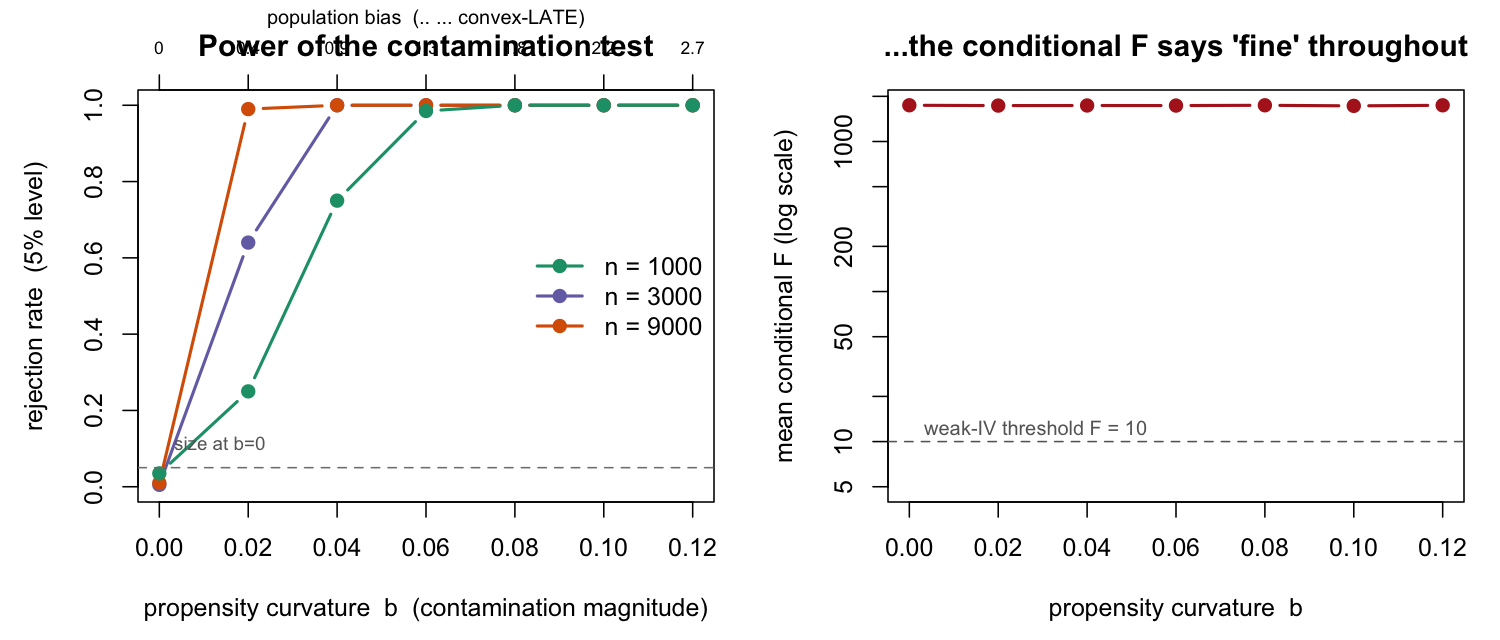
\includegraphics[width=\textwidth]{../figures/iv_power_curve.png}
\caption{Left panel. Rejection rate of the directed test vs.\ propensity
curvature $b$ (bottom axis) and induced population bias (top axis), for
$n\in\{1000,3000,9000\}$, with the dashed line at the $5\%$ level. Right panel.
The mean conditional $F$ (log scale) is invariant to $b$, sitting near
$\num{1740}$ throughout.}
\label{fig:power}
\end{figure}

\begin{table}[h]\centering
\caption{Power curve. Rejection rates ($5\%$ level, $200$ replications, $B=99$)
by curvature knob $b$ and sample size. Induced population bias
$\beta_{2SLS}-\bar L$ at $n=\num{200000}$. Mean conditional $F$ at $n=9000$.}
\label{tab:power}
\begin{tabular}{rrrrrr}
\toprule
$b$ & bias & $n=1000$ & $n=3000$ & $n=9000$ & mean cond.\ $F$\\
\midrule
0.00 & $-0.00$ & 0.035 & 0.005 & 0.010 & \num{1744}\\
0.02 & 0.42    & 0.250 & 0.640 & 0.990 & \num{1736}\\
0.04 & 0.85    & 0.750 & 1.000 & 1.000 & \num{1738}\\
0.06 & 1.33    & 0.985 & 1.000 & 1.000 & \num{1736}\\
0.08 & 1.79    & 1.000 & 1.000 & 1.000 & \num{1744}\\
0.10 & 2.22    & 1.000 & 1.000 & 1.000 & \num{1728}\\
0.12 & 2.68    & 1.000 & 1.000 & 1.000 & \num{1743}\\
\bottomrule
\end{tabular}
\end{table}

\begin{table}[h]\centering
\caption{Directed-S vs.\ Directed-X as instrument--covariate collinearity rises,
in the contaminated design (rejection $=$ power, the bias it faces in the third
column) and the harmless design (rejection $=$ size, $5\%$ nominal). $300$
replications, $n=3000$, cubic basis. Directed-S false-alarms in every harmless row
because it tests the sufficient condition $\theta=0$. Directed-X keeps full power
against genuine bias and holds size throughout, so the pairs bootstrap protects it
against the weak-identification caveat of Corollary~\ref{cor:frontier} over this
range.}
\label{tab:svx}
\begin{tabular}{rrccccc}
\toprule
 & & \multicolumn{3}{c}{Contaminated (power)} & \multicolumn{2}{c}{Harmless (size)}\\
\cmidrule(lr){3-5}\cmidrule(lr){6-7}
$\kappa$ & $\Var(Z\mid X)$ & bias & Directed-S & Directed-X & Directed-S & Directed-X\\
\midrule
0.5  & 0.230 & 2.54 & 1.00 & 1.00 & 1.00 & 0.040\\
2.0  & 0.119 & 6.27 & 1.00 & 1.00 & 1.00 & 0.050\\
8.0  & 0.027 & 7.81 & 1.00 & 1.00 & 1.00 & 0.047\\
16.0 & 0.014 & 7.85 & 1.00 & 1.00 & 1.00 & 0.030\\
\bottomrule
\end{tabular}
\end{table}

\begin{table}[h]\centering
\caption{Contamination share. Population value, plug-in estimate at $n=3000$,
$95\%$ percentile-bootstrap coverage of the population share ($250$ replications,
$B=149$), and the induced 2SLS bias.}
\label{tab:share}
\begin{tabular}{rrrrr}
\toprule
$\kappa$ & $\varrho$ (pop.) & $\hat\varrho$ ($n{=}3000$) & $95\%$ coverage & bias\\
\midrule
0.25 & 0.022 & 0.023 & 0.928 & 1.283\\
0.50 & 0.078 & 0.079 & 0.936 & 2.501\\
1.00 & 0.240 & 0.238 & 0.936 & 4.363\\
2.00 & 0.495 & 0.495 & 0.944 & 6.297\\
4.00 & 0.680 & 0.684 & 0.964 & 7.428\\
8.00 & 0.741 & 0.741 & 0.948 & 7.853\\
16.0 & 0.754 & 0.756 & 0.924 & 7.910\\
\bottomrule
\end{tabular}
\end{table}

\begin{figure}[h]\centering
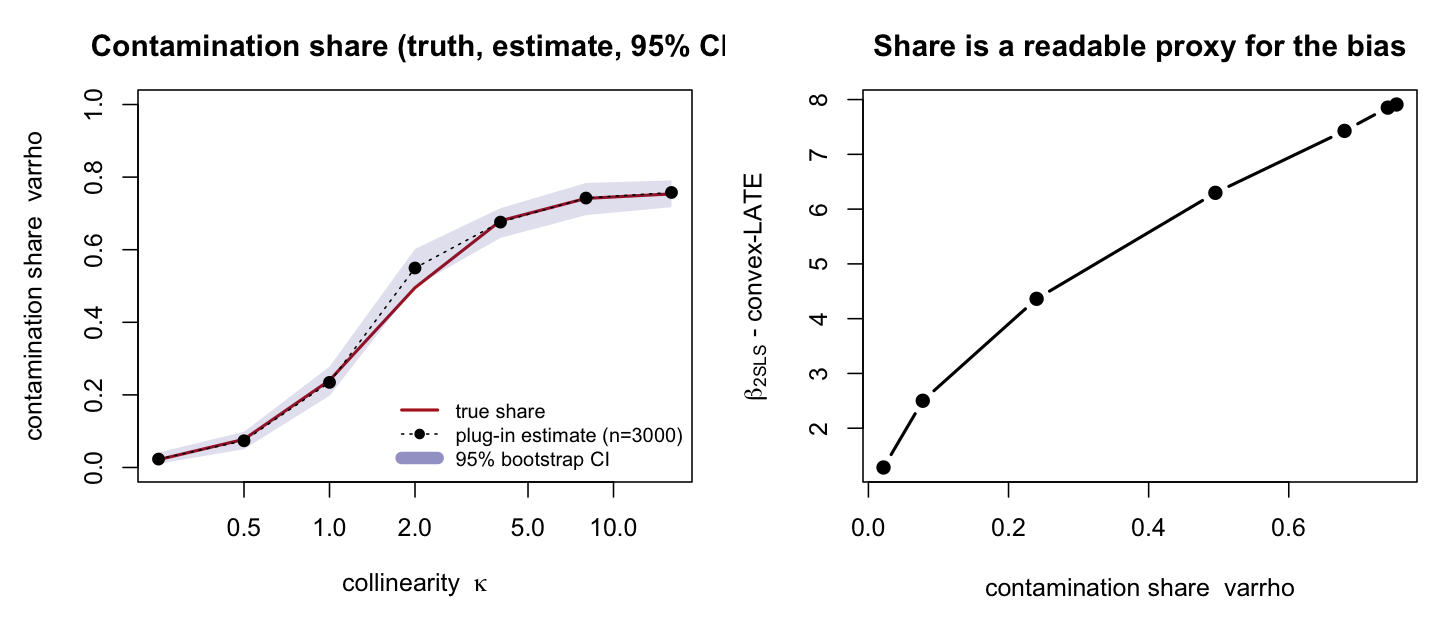
\includegraphics[width=\textwidth]{../figures/iv_contamination_share.png}
\caption{Left panel. The population contamination share (solid), the plug-in
estimate at $n=3000$ (points) and its $95\%$ bootstrap band, against the
collinearity knob $\kappa$. Right panel. Along this one-parameter family the
population bias is monotone in the share, so here $\hat\varrho$ orders these designs
by danger. This ordering is a feature of the family swept, not a general property.
Across unrelated designs bias also depends on $\theta_Y$ and $\bar L$, so equal
shares can accompany different biases.}
\label{fig:share}
\end{figure}

%=============================================================================
\begin{thebibliography}{99}
%=============================================================================

\bibitem[Andrews et~al.(2019)]{andrews2019}
Andrews, I., Stock, J.H., Sun, L., 2019. Weak instruments in instrumental
variables regression: theory and practice. Annual Review of Economics 11,
727--753.

\bibitem[Angrist et~al.(1996)]{angrist1996}
Angrist, J.D., Imbens, G.W., Rubin, D.B., 1996. Identification of causal effects
using instrumental variables. Journal of the American Statistical Association 91,
444--455.

\bibitem[Abadie(2003)]{abadie2003}
Abadie, A., 2003. Semiparametric instrumental variable estimation of treatment
response models. Journal of Econometrics 113, 231--263.

\bibitem[Acemoglu et~al.(2001)]{acemoglu2001}
Acemoglu, D., Johnson, S., Robinson, J.A., 2001. The colonial origins of
comparative development: an empirical investigation. American Economic Review 91,
1369--1401.

\bibitem[Angrist and Lavy(1999)]{angrist1999}
Angrist, J.D., Lavy, V., 1999. Using Maimonides' rule to estimate the effect of
class size on scholastic achievement. Quarterly Journal of Economics 114, 533--575.

\bibitem[Bierens(1990)]{bierens1990}
Bierens, H.J., 1990. A consistent conditional moment test of functional form.
Econometrica 58, 1443--1458.

\bibitem[Card(1995)]{card1995}
Card, D., 1995. Using geographic variation in college proximity to estimate the
return to schooling, in: Aspects of Labour Market Behaviour. University of Toronto
Press, pp.~201--222.

\bibitem[Cornwell and Trumbull(1994)]{cornwell1994}
Cornwell, C., Trumbull, W.N., 1994. Estimating the economic model of crime with
panel data. Review of Economics and Statistics 76, 360--366.

\bibitem[Mroz(1987)]{mroz1987}
Mroz, T.A., 1987. The sensitivity of an empirical model of married women's hours
of work to economic and statistical assumptions. Econometrica 55, 765--799.

\bibitem[Poterba et~al.(1995)]{poterba1995}
Poterba, J.M., Venti, S.F., Wise, D.A., 1995. Do 401(k) contributions crowd out
other personal saving? Journal of Public Economics 58, 1--32.

\bibitem[Romer(1993)]{romer1993}
Romer, D., 1993. Openness and inflation: theory and evidence. Quarterly Journal of
Economics 108, 869--903.

\bibitem[Wooldridge(2010)]{wooldridge2010}
Wooldridge, J.M., 2010. Econometric Analysis of Cross Section and Panel Data, 2nd
ed. MIT Press.

\bibitem[Blandhol et~al.(2022)]{blandhol2022}
Blandhol, C., Bonney, J., Mogstad, M., Torgovitsky, A., 2022. When is TSLS
actually LATE? NBER Working Paper 29709.

\bibitem[Goldsmith-Pinkham et~al.(2024)]{goldsmith2024}
Goldsmith-Pinkham, P., Hull, P., Koles{\'a}r, M., 2024. Contamination bias in
linear regressions. American Economic Review 114, 4015--4051.

\bibitem[Zhao et~al.(2025)]{ddl2025}
Zhao, A., Ding, P., Li, F., 2025. Two-stage least squares with treatment--covariate
interactions for treatment effect heterogeneity. Working paper, arXiv:2502.00251.

\bibitem[Krumme and Westphal(2026)]{krumme2026}
Krumme, A., Westphal, M., 2026. Testing IV validity and LATE interpretation using
flexible covariate specifications. IZA Discussion Paper 18573.

\bibitem[Dossani et~al.(2024)]{dossani2024}
Dossani, A., Dotson, J.P., Schonlau, R., 2024. Contaminated control variables in
2SLS models. Working paper.

\bibitem[S{\l}oczy{\'n}ski et~al.(2026)]{ssu2026}
S{\l}oczy{\'n}ski, T., Sun, L., Uysal, S.D., 2026. A practical guide to
instrumental variables methods with heterogeneous treatment effects. Working
paper, arXiv:2605.15115.

\bibitem[Young(2024)]{young2024}
Young, A., 2024. Nearly collinear robust procedures for 2SLS estimation. The Stata
Journal 24, 3--28.

\bibitem[van der Vaart(1998)]{vandervaart1998}
van der Vaart, A.W., 1998. Asymptotic Statistics. Cambridge University Press.

\bibitem[Bound et~al.(1995)]{bound1995}
Bound, J., Jaeger, D.A., Baker, R.M., 1995. Problems with instrumental variables
estimation when the correlation between the instruments and the endogenous
explanatory variable is weak. Journal of the American Statistical Association 90,
443--450.

\bibitem[Chernozhukov et~al.(2018)]{chernozhukov2018}
Chernozhukov, V., Chetverikov, D., Demirer, M., Duflo, E., Hansen, C., Newey, W.,
Robins, J., 2018. Double/debiased machine learning for treatment and structural
parameters. The Econometrics Journal 21, C1--C68.

\bibitem[Conley et~al.(2012)]{conley2012}
Conley, T.G., Hansen, C.B., Rossi, P.E., 2012. Plausibly exogenous. Review of
Economics and Statistics 94, 260--272.

\bibitem[de Chaisemartin(2017)]{dechaisemartin2017}
de Chaisemartin, C., 2017. Tolerating defiance? Local average treatment effects
without monotonicity. Quantitative Economics 8, 367--396.

\bibitem[Heckman and Vytlacil(2005)]{heckman2005}
Heckman, J.J., Vytlacil, E., 2005. Structural equations, treatment effects, and
econometric policy evaluation. Econometrica 73, 669--738.

\bibitem[Imbens and Angrist(1994)]{imbens1994}
Imbens, G.W., Angrist, J.D., 1994. Identification and estimation of local average
treatment effects. Econometrica 62, 467--475.

\bibitem[van Kippersluis and Rietveld(2018)]{kippersluis2018}
van Kippersluis, H., Rietveld, C.A., 2018. Beyond plausibly exogenous. The
Econometrics Journal 21, 316--331.

\bibitem[Mogstad and Torgovitsky(2018)]{mogstad2018}
Mogstad, M., Torgovitsky, A., 2018. Identification and extrapolation of causal
effects with instrumental variables. Annual Review of Economics 10, 577--613.

\bibitem[Mogstad and Torgovitsky(2024)]{mogstad2024}
Mogstad, M., Torgovitsky, A., 2024. Instrumental variables with unobserved
heterogeneity in treatment effects, in: Handbook of Labor Economics. Elsevier.

\bibitem[Montiel Olea and Pflueger(2013)]{montielolea2013}
Montiel Olea, J.L., Pflueger, C., 2013. A robust test for weak instruments.
Journal of Business \& Economic Statistics 31, 358--369.

\bibitem[Newey(1985)]{newey1985}
Newey, W.K., 1985. Maximum likelihood specification testing and conditional
moment tests. Econometrica 53, 1047--1070.

\bibitem[Newey and McFadden(1994)]{newey1994}
Newey, W.K., McFadden, D., 1994. Large sample estimation and hypothesis testing,
in: Handbook of Econometrics, vol.~4. Elsevier, pp.~2111--2245.

\bibitem[Ramsey(1969)]{ramsey1969}
Ramsey, J.B., 1969. Tests for specification errors in classical linear
least-squares regression analysis. Journal of the Royal Statistical Society B 31,
350--371.

\bibitem[Sanderson and Windmeijer(2016)]{sanderson2016}
Sanderson, E., Windmeijer, F., 2016. A weak instrument $F$-test in linear IV
models with multiple endogenous variables. Journal of Econometrics 190, 212--221.

\bibitem[S{\l}oczy{\'n}ski(2022)]{sloczynski2022}
S{\l}oczy{\'n}ski, T., 2022. When should we (not) interpret linear IV estimands
as LATE? Working paper, Brandeis University.

\bibitem[Staiger and Stock(1997)]{staiger1997}
Staiger, D., Stock, J.H., 1997. Instrumental variables regression with weak
instruments. Econometrica 65, 557--586.

\bibitem[Stock and Yogo(2005)]{stock2005}
Stock, J.H., Yogo, M., 2005. Testing for weak instruments in linear IV
regression, in: Identification and Inference for Econometric Models. Cambridge
University Press, pp.~80--108.

\bibitem[Tauchen(1985)]{tauchen1985}
Tauchen, G., 1985. Diagnostic testing and evaluation of maximum likelihood
models. Journal of Econometrics 30, 415--443.

\end{thebibliography}

\end{document}
